\documentclass[letterpaper, 10pt, conference]{ieeeconf}
\IEEEoverridecommandlockouts \overrideIEEEmargins
\usepackage{amsmath,amssymb,url,times,subfigure,graphicx,theorem}
\usepackage{graphicx,subfigure,hyperref}
\usepackage{color,comment}
\usepackage{csquotes}
%\usepackage{refcheck}

\usepackage{epic,eepic}

\usepackage[]{algorithm2e}
%\usepackage{algorithmicx}
%\usepackage{algpseudocode}

%\usepackage{algorithm}
%\usepackage{algpseudocode}
%\usepackage{pifont}



%\usepackage{amsmath}
%\usepackage{algorithm}
%\usepackage[noend]{algpseudocode}
%
%\makeatletter
%\def\BState{\State\hskip-\ALG@thistlm}
%\makeatother

%\definecolor{red}{rgb}{0,0,0}

\newcommand{\norm}[1]{\ensuremath{\left\| #1 \right\|}}
\newcommand{\abs}[1]{\ensuremath{\left| #1 \right|}}
\newcommand{\bracket}[1]{\ensuremath{\left[ #1 \right]}}
\newcommand{\braces}[1]{\ensuremath{\left\{ #1 \right\}}}
\newcommand{\parenth}[1]{\ensuremath{\left( #1 \right)}}
\newcommand{\ip}[1]{\ensuremath{\langle #1 \rangle}}
\newcommand{\refeqn}[1]{(\ref{eqn:#1})}
\newcommand{\reffig}[1]{Fig. \ref{fig:#1}}
\newcommand{\tr}[1]{\mbox{tr}\ensuremath{\negthickspace\bracket{#1}}}
\newcommand{\trs}[1]{\mbox{tr}\ensuremath{\!\bracket{#1}}}
\newcommand{\deriv}[2]{\ensuremath{\frac{\partial #1}{\partial #2}}}
\newcommand{\G}{\ensuremath{\mathsf{G}}}
\newcommand{\SO}{\ensuremath{\mathsf{SO(3)}}}
\newcommand{\T}{\ensuremath{\mathsf{T}}}
\renewcommand{\L}{\ensuremath{\mathsf{L}}}
\newcommand{\so}{\ensuremath{\mathfrak{so}(3)}}
\newcommand{\SE}{\ensuremath{\mathsf{SE(3)}}}
\newcommand{\se}{\ensuremath{\mathfrak{se}(3)}}
\renewcommand{\Re}{\ensuremath{\mathbb{R}}}
\newcommand{\Sph}{\ensuremath{\mathsf{S}}}
\newcommand{\aSE}[2]{\ensuremath{\begin{bmatrix}#1&#2\\0&1\end{bmatrix}}}
\newcommand{\ase}[2]{\ensuremath{\begin{bmatrix}#1&#2\\0&0\end{bmatrix}}}
\newcommand{\D}{\ensuremath{\mathbf{D}}}
\renewcommand{\d}{\ensuremath{\mathbf{d}}}
\newcommand{\pair}[1]{\ensuremath{\left\langle #1 \right\rangle}}
\newcommand{\met}[1]{\ensuremath{\langle\!\langle #1 \rangle\!\rangle}}
\newcommand{\Ad}{\ensuremath{\mathrm{Ad}}}
\newcommand{\ad}{\ensuremath{\mathrm{ad}}}
\newcommand{\g}{\ensuremath{\mathfrak{g}}}

\title{\LARGE \bf
Bayesian Occupancy Grid Mapping via an Exact Inverse Sensor Model}

\author{Evan Kaufman, Taeyoung Lee, Zhuming Ai, and Ira S. Moskowitz%
\thanks{Evan Kaufman, Taeyoung Lee, Mechanical and Aerospace Engineering, George Washington University, Washington DC 20052 {\tt \{evankaufman,tylee\}@gwu.edu}}
\thanks{Zhuming Ai, Ira S. Moskowitz, Information Management \& Decision Architectures, U.S. Naval Research Laboratory,  Washington, DC 20375}
\thanks{This research has been supported by the U.S. Naval Research Laboratory Base Program Work Unit ``Intelligent Microflyer'' and in part by NSF under the grants CMMI-1243000, CMMI-1335008, and CNS-1337722.}
}


\newcommand{\EditEK}[1]{{\color{blue}\protect #1}}
%\renewcommand{\EditTL}[1]{{\protect #1}}


\newtheorem{definition}{Definition}
\newtheorem{lem}{Lemma}
\newtheorem{prop}{Proposition}
\newtheorem{cor}{Corollary}
\newtheorem{remark}{Remark}



\begin{document}
\allowdisplaybreaks


\maketitle \thispagestyle{empty} \pagestyle{empty}

\begin{abstract}
Occupancy grid maps are spatial representations of environments, where the space of interest is decomposed into a number of cells that are considered either occupied or free. This paper focuses on occupancy grid mapping, which is to estimate the probability of occupancy for each cell based on range measurements from a known location. For a given probabilistic model of a range sensor, we propose a computationally efficient method to obtain an exact inverse sensor model, and it is utilized to construct a probabilistic mapping algorithm according to the Bayesian framework. Compared with the existing occupancy grid mapping techniques that rely on approximate inverse sensor models, the proposed approach yields substantially more accurate maps for the same set of measurements. These are illustrated by numerical examples and experiments. 
\end{abstract}

\section{Introduction}

Mapping in the context of robotics is to generate maps, which represents the environment in close proximity of a robot. This problem is crucial to understanding the surrounding regions when a robot enters an uncertain environment.
Various map representations have been applied to the mapping problem such as occupancy grids~\cite{WolSuk05}, octomaps~\cite{WurHorBenStaBur10}, or feature-based maps%in a landmark representation
~\cite{MonThrKolWeg02}.
%To build maps in real time, a computationally-efficient algorithm is required.% \EditTL{rewrite this paragraph for mapping, without introducing SLAM here}

This paper focusses on the popular occupancy grid representation, where the map space is decomposed into evenly-spaced grid cells that are considered as either occupied or free.
The \emph{inverse sensor model} is the probability of occupancy for a grid cell based on range measurements and the configuration of the mobile robot, which is of fundamental importance with occupancy grid mapping. However, the exact solution to the inverse sensor model has not been utilized in occupancy grid mapping, because the computational requirements are too cumbersome to compute the exact model in real time~\cite{ThrBurFox05}.

Instead, several techniques have been proposed to approximate the exact inverse sensor model. %Due to the computational limitations, two common approaches are applied to obtain a function close to the inverse sensor model.
In the early occupancy grid mapping applications based on sonar sensors, \emph{ad hoc} techniques are employed to obtain an inverse sensor model, where the bearings of depth measurements are considered uncertain because the directions of bouncing sound waves are highly inaccurate~\cite{MorElf85,Elf89}.
%These occupancy grid mapping schemes employ \emph{ad hoc} techniques to obtain the inverse sensor model.
These techniques are based on approximate functions to represent the inverse sensor model with questionable accuracy~\cite{ChoLynHutKanBurKavThr05} and applied to more modern sensors in~\cite{And09},~\cite{PirRutBisSch11}.

The other popular approach to obtain an approximate inverse sensor model is to simulate maps, robot poses, and measurements and use a learning algorithm, to approximate the inverse sensor model~\cite{Thr01,ThrBurFox05}. These approaches are undesirable in practice due to complexities associated to implementing a learning algorithm. For example, the accuracy of such inverse sensor models strongly depends on the samples selected for learning, but it is unclear how to select those samples, or how many samples are required to obtain a reasonable approximation. Furthermore, it is challenging to apply any learning algorithm over the large dimensional space composed of maps, poses, and measurements. 

%and they only yield probabilistic approximations without strong mathematical justification. 

%These approaches simply treat occlusions with discrete probabilities of detection, regardless of whether one cell may completely, partially, or not block another cell in the sensor field of view.

%Furthermore, both approaches follow a log-odds ratio Bayesian framework, imposing an additional Markov assumption.

%These techniques are not also suitable for modern range sensor with the highly accurate bearing~\cite{Thr03}. Based on recent improvements in sensor technology, the occupancy grid mapping problem has been restructured using the fact that depth measurement bearings are known. \EditTL{do we need this paragraph?}

This paper proposes a computationally efficient algorithm to construct the exact inverse sensor model. More explicitly, for a given forward sensor model defined by the probability distribution of range measurements, this algorithm yields the a posteriori probability of occupancy of all the cells within the area covered by the range sensor from the range measurements. The key idea is reducing the computational load by using the fact that if a cell is occupied, the occupancy of the other cells blocked by it is irrelevant to the forward sensor model, and this model is systematically utilized with various probabilistic properties to derive a computationally-efficient solution to the inverse sensor model. Furthermore, the proposed approach integrates a priori probability of occupancy and multiple range measurements according to the Bayesian framework to obtain more accurate maps. As such, it contrasts from the existing framework based on log-odds ratios that impose an additional Markov assumption. 

%these are constructed 

In short, the main contribution of this paper is proposing the exact inverse sensor model and constructing a Bayesian occupancy grid mapping based on that. Compared with the current mapping algorithms based on an approximate inverse sensor model, this approach yields more accurate occupancy probabilities. This constructs substantially more accurate occupancy grid maps with less uncertainty for the same set of measurements, and these are directly illustrated by numerical examples and preliminary experimental results. While this paper is focused on the mapping problem in two-dimensional environments, the presented results can be certainly utilized in SLAM or stochastic motion planning in three dimensions.


%occupancy probabilities that are more accurate than prior work, which may be applied for more accurate real-time map generation in the SLAM problem and more effective trajectory planning strategies based on map uncertainty.

The paper is organized as follows.
The problem is formulated in Section \ref{sec:ProbForm}, and the exact solution to the occupancy grid mapping problem is derived in Section \ref{sec:ISM}.
A numerical result shows the improved accuracy in Section \ref{sec:NumRes}, and an experimental result with the Kinect depth sensor shows the improvement in map certainty in Section \ref{sec:ExpRes}, followed by conclusions.


\section{Problem Formulation}
\label{sec:ProbForm}

\subsection{Range Sensor}

Consider a range sensor that provides scans of the surrounding environment to identify the closest occupied space. The location and the direction of the sensor, referred to as the \emph{pose} at time $t$ is denoted by $X_t$. The range sensor returns a measurement \emph{scan} $Z_t$, which is composed of $n_z$ measurement \emph{rays} $z_{t,1},z_{t,2},...,z_{t,n_z}$. The $l$-th measurement ray for $l\in\braces{1,2,...,n_z}$ contains the depth (range) and bearing (direction) of a small region inside the sensor field of view (FOV) that corresponds to a circular sector. For a given $X_t$, it is assumed that the origin and the direction of each ray is known deterministically.

The probability density function, namely $p(z_{t,l}|m,X_t)$ with respect to the depth of the $l$-th measurement ray conditioned on the map $m$ and the pose $X_t$ is commonly referred to as the \emph{forward sensor model}, which characterizes the corresponding depth sensor, such as the maximum range or accuracy. The forward sensor model satisfies  (i) the ranges of all depth measurements are positive and finite, and (ii) measurement rays cannot pass through occupied regions.

Throughout this paper, it is assumed that the forward sensor model of the selected sensor is given. This can be determined empirically or analytically. For example, the \emph{beam model for range finders} satisfying  the above criteria is described in~\cite{ThrBurFox05}.
%, which contains Gaussian, exponential, uniform, and point pass portions~\cite{ThrBurFox05}.
%At time $t$ and given the pose $X_t$ and map $m$, the beam model with respect to the $l$-th measurement ray $z_{t,l}$ is the probability density defined as
%\begin{align}
%p(z_{t,l})=\begin{cases}
%\frac1{z_{max}-z_{min}}P_{hit}+P_{short}+P_{rand}\ \text{if},\ 
%\\
%P_{max},
%\end{cases}
%\end{align}
%where $z_{min}\leq z_{t,l}\leq z_{max}$ and $\hat z_{t,l}$ is the distance between the robot and the closest occupied location along the direction $z_{t,l}$.
%The probabilities are defined such that $P_{hit}$ is the probability of the depth originating from this occupied location (Gaussian), $P_{exp}$ is the probability that an unexpected occlusion blocks the first occupied location of the map (exponential), $P_{rand}$ is the probability of a phantom reading (uniform), and $P_{max}$ is the probability that the sensor returns its maximum value (point mass).
%These probabilities are normalized such that
%\begin{align}
%P_{hit}+P_{short}+P_{rand}+P_{max}=1.
%\end{align}

%We assume that this forward sensor model depends on the closest occupied location, and is independent of the occupancy beyond this point.
	
\subsection{Occupancy Grid Mapping}

Let a map $m$ be decomposed into $n_m$ evenly-spaced grid cells, where the $i$-th grid cell is assigned to a static binary random variable $\mathbf{m}_i$ for $i\in\braces{1,2,...,n_m}$, that is defined as $\mathbf{m}_i=1$ when it is occupied, and $\mathbf{m}_i=0$ when it is free. The location and size of each grid cell is assumed to be known. Therefore, a map $m$ is defined by $\{\mathbf{m}_1,\ldots, \mathbf{m}_{n_m}\}$, and there are $2^{n_{m}}$ possible maps. 

Another random variable is defined as $\bar{\mathbf{m}}_i=1-\mathbf{m}_i$ for convenience. The probability that the $i$-th cell is occupied is $P(\mathbf{m}_i)$, and the probability that it is free is $P(\bar{\mathbf{m}}_i)=1-P(\mathbf{m}_i)$. The random variables $\mathbf{m}_i$ are mutually independent, 
\begin{align}
P(m)=P(\mathbf{m}_1,\mathbf{m}_2,...,\mathbf{m}_{n_m})=\prod_{i=1}^{n_m}P(\mathbf{m}_i).
\end{align}

%Occupancy grid mapping produces a probabilistic map; none of the $n_m$ grid cell occupancies are completely certain.
Occupancy grid mapping  is to determine these probabilities based on robot poses and measurement scans. More explicitly, let $X_{1:t}$ denote the history of poses from the initial time to the current time, $\{X_1,X_2,\ldots, X_t\}$, and let $Z_{1:t}$ be the measurement history. The goal is to obtain $P(\mathbf{m}_i|X_{1:t},Z_{1:t})$, commonly referred to as the \emph{inverse sensor model} for given forward sensor model $p(z|m,X)$ and the initial estimate of the map $P(m)$ with $X_{1:t}$ and $Z_{1:t}$.

	% Def of occupancy grid
	% Cell occupancies are assumed independent
	% Probabilistic maps
	% Notations
	% Mapping problem
	
\subsection{Mapping via Log-Odds Ratio}

One of the popular frameworks of updating binary random variables with static state is with a binary Bayesian filter using the log-odds ratio formulation.
The main idea is that instead of multiplying terms from prior and current time steps, the properties of logarithms allow these terms to be simply added, while avoiding truncation issues associated with probabilities close to $0$ or $1$~\cite{ThrBurFox05}.
The log-odds ratio is also popular because learning techniques with forward models~\cite{Thr01},~\cite{Thr03} or ad hoc techniques~\cite{MorElf85},~\cite{Elf89} are simpler to derive when they need not consider $P(\mathbf{m}_i|X_{1:t},Z_{1:t-1})$ as part of the inverse sensor model, but rather only $P(\mathbf{m}_i)$, which is typically fixed and uniform for all cells.

However, the log-odds ratio formulation makes an assumption that is not consistent with the occupancy grid mapping problem. It is assumed that if $X_t$ and $\mathbf{m}_i$ are known, then $Z_t$ is independent of $X_{1:t-1}$ and $Z_{1:t-1}$, i.e.,
%\begin{align}
%\label{eqn:FirstBayesRule}
%P(\mathbf{m}_i|X_{1:t},Z_{1:t})
%&
%=\frac{P(Z_t|\mathbf{m}_i,X_{1:t},Z_{1:t-1})P(\mathbf{m}_i|X_{1:t},Z_{1:t-1})}{P(Z_t|X_{1:t},Z_{1:t-1})}.
%\end{align}
\begin{align}
\label{eqn:AssumptionEarly}
P(Z_t|\mathbf{m}_i,X_{1:t},Z_{1:t-1})\approx P(Z_t|\mathbf{m}_i,X_t).
\end{align}
The above equation can be justified if both sides are conditioned by the complete map $m$ instead of just the cell $\mathbf{m}_i$, since the probability distribution of the sensor is completely determined by its pose and the map through the forward sensor model. However, since it is conditioned only by the $i$-th cell, past poses $X_{1:t-1}$ and past measurement scans $Z_{1:t-1}$ may have certain information about the occupancy of the other cells, which should be considered in calculating the probability distribution of the measurement scan $Z_t$.  In short, this log-odds ratio framework is based on the assumption that neglects potentially important information contained in $X_{1:t-1}$ and $Z_{1:t-1}$.


%However, past poses $X_{1:t-1}$ and past measurement scans $Z_{1:t-1}$ may suggest that there exist occupied regions that occlude some or all of $Z_t$ from detecting $\mathbf{m}_i$ from the current pose $X_t$.
%Since this assumption neglects potentially important information contained in $X_{1:t-1}$ and $Z_{1:t-1}$, this framework is subject to poor results.
%Hence, the log-odds ratio formulation is completely avoided in further analysis.


	
	% approximated inverse sensor model
	% markov assumption
	% shortcoming, reason this is avoided
	
\section{Exact Inverse Sensor Model}
\label{sec:ISM}

Due to the computational complexity, approximate inverse sensor models have been used for occupancy grid mapping with simplifying assumptions. In this section, we propose an algorithm to compute the exact inverse sensor model efficiently. 
%Much like the forward sensor model that reasons measurements from a known map, he inverse sensor model reasons that map from known measurements~\cite{ThrBurFox05}.
%While the inverse sensor model varies slightly in meaning in numerous publications, two versions are derived in this paper, both based on a Bayesian framework.
We present two versions according to Bayesian framework. The first type is referred to as the \emph{ray inverse sensor model} $P(\mathbf{m}_i|X_{1:t},Z_{1:t-1},z_{t,l})$, which only considers $l$-th ray at time $t$, i.e., one-dimensional inverse sensor model. The second type is referred to as the \emph{scan inverse sensor model} $P(\mathbf{m}_i|X_{1:t},Z_{1:t})$, which combines the information from \emph{all} measurement rays \emph{simultaneously} at the $t$-th time step for two-dimensional cases. These are developed in a sequential form to be repeated at each time step.


%These are contrary to inverse sensor models commonly used with the log-odds ratio formulations, and the proposed algorithm integrates all of past poses and measurement scans with the current ones to obtain more accurate estimate of the map.

\subsection{Ray Inverse Sensor Model}

Suppose the probability of the map conditioned on the past poses and measurements, namely $P(m|X_{1:t-1},Z_{1:t-1})$, is known. Here we construct a posteriori probability $P(m|z_{t,l},X_{1:t},Z_{1:t-1})$, based on the current pose $X_t$, the measurement from the $l$-th ray $z_{t,l}$, and the given forward sensor model $p(z_{t_l}|m,X_t)$.

\paragraph{Bayesian Framework}
%Assuming that the probability density of thxe sensor measurement is fixed over a small measurement region $\Delta z$, 
Bayes' rule yields
%First, Bayes' rule is applied for a particular map $m$ and arbitrarily small measurement region $\Delta z$, yielding
\begin{align}
\label{eqn:BayesRuleRayISM}
P(&m|z_{t,l},X_{1:t},Z_{1:t-1})\nonumber
\\
&=\frac{p(z_{t,l}|m,X_{1:t},Z_{1:t-1})P(m|X_{1:t-1},Z_{1:t-1})}{p(z_{t,l}|X_{1:t},Z_{1:t-1})},
\end{align}
where we have used the fact that $X_t$ carries no information about $m$ without $Z_t$.
If the current pose $X_t$ and map $m$ are known, then the measurement ray $z_{t,l}$ is independent of past poses $X_{1:t-1}$ and past measurements $Z_{1:t-1}$ to obtain
%Note that this is contrary to approaches that consider $X_t$ and $\mathbf{m}_i$ (not the full map $m$) as enough information, ignoring the occupancy of other cells in this term.
%Then, \refeqn{BayesRuleRayISM} can be rewritten as
\begin{align}
P(m|z_{t,l},&X_{1:t},Z_{1:t-1})\nonumber
\\
&
=\eta_{t,l}p(z_{t,l}|m,X_{t})P(m|X_{1:t-1},Z_{1:t-1}),
\end{align}
where the normalizing constant $\eta_{t,l}\in\Re$ absorbs all terms independent of the map $m$.

%Assuming $z_{t,l}$ measures an occupied cell, then $z_{t,l}$ may be a result of the occupancy of $\mathbf{m}_i$, or $z_{t,l}$ may measure a different occupied cell.

Next, we compute the occupancy probability of each cell. Let $\mathcal{M}_i$ be the set of maps where the $i$-th cell is occupied, i.e., $\mathcal{M}_i =\{m\in\{0,1\}^{{n_m}}\,|\ \mathbf{m}_i=1\}$. To compute the probability of occupancy of the $i$-th cell, all possible combinations of map in $\mathcal{M}_i$ should be considered, i.e., 
%All possible combinations of map $m$ must be considered in which $\mathbf{m}_i$ is occupied, denoted as $m:m(i)=\mathbf{m}_i$,
\begin{align}
\label{eqn:InvSenModWithProbDens}
&P(\mathbf{m}_i|z_{t,l},X_{1:t},Z_{1:t-1})\nonumber
\\
&=\eta_{t,l}\sum_{m\in\mathcal{M}_i}p(z_{t,l}|m,X_{t})P(m|X_{1:t-1},Z_{1:t-1}).
\end{align}
Furthermore, to determine the normalizing constant $\eta_{t,l}$, the complement $P(\bar{\mathbf{m}}_i|z_{t,l},X_{1:t},Z_{1:t-1})$ must be calculated in the similar manner. Since there are $2^{n_{m}-1}$ maps in $\mathcal{M}_i$, these equations require $2^{n_m}$ terms to compute the summation for the $i$-th grid cell, and it should be repeated for other cells. This is the main reason why the current results are based on certain approximations of the above expression. 

	
\paragraph{Computationally Efficient Approach}

In this paper, we propose a computational algorithm to evaluate \refeqn{InvSenModWithProbDens} efficiently. 
Since the cells outside of the sensor FOV are not affected, we focus on a reduced map $r_l$ in the FOV of the $l$-th ray. This reduced map is chosen such that each cell of $r_l$ corresponds to a grid cell of $m$ that the $l$-th ray intersects, ordered by increasing distance, which is easily determined from geometry. Let $\mathbf{r}_{l,k}$ be the binary random variable representing the occupancy of the $k$-th cell of the $l$-th ray. The number of cells in the reduced map is denoted by $n_{r,l}\leq n_m$.

Next, let $\mathbf{r}_{l,k+}$ correspond to the set of maps that the $k$-th cell of the $l$-th ray is occupied, cells with lower index are free, and cells with greater index may or may not be occupied. In other words, the $k$-th cell $\mathbf{r}_{l,k}$ is the closest occupied cell to current pose $X_t$ along the $l$-th ray. Then, the forward sensor model is identical for all maps defined by $\mathbf{r}_{l,k+}$, regardless of the occupancy of the cells beyond the $k$-th cell, and the corresponding forward sensor model $p(z_{t,l}|\mathbf{r}_{l,k+},X_{t})$ depends on the distance from $X_t$ to the $k$-th cell. Based on this, we present the following computational algorithm to compute the inverse sensor model.

\begin{prop}
For the $l$-th measurement ray, the a posteriori probability of the occupancy of the $k$-th cell, namely the ray inverse sensor model is given by
\begin{align}
\label{eqn:RayISMAnswer}
P(\mathbf{r}_{l,k}|z_{t,l},X_{1:t},Z_{1:t-1})&=\eta_{t,l}\tilde P(\mathbf{r}_{l,k}|z_{t,l},X_{1:t},Z_{1:t-1}),
\end{align}
where the unnormalized probability of the inverse sensor model is defined as
\begin{align}
\label{eqn:Unnormalized}
& \tilde P(\mathbf{r}_{l,k}|z_{t,l},X_{1:t},Z_{1:t-1})\nonumber\\
&=P(\mathbf{r}_{l,k}|X_{1:t-1},Z_{1:t-1})\nonumber\\
&\quad\times 
\bigg[\sum_{i=1}^{k-1}\bigg\{\prod_{j=0}^{i-1}P(\bar{\mathbf{r}}_{l,j}|X_{1:t-1},Z_{1:t-1})\bigg\}\nonumber\\
&\quad\times p(z_{t,l}|\mathbf{r}_{l,i+},X_t)P(\mathbf{r}_{l,i}|X_{1:t-1},Z_{1:t-1})\bigg]\nonumber\\
&\quad + \bigg\{\prod_{j=0}^{k-1}P(\bar{\mathbf{r}}_{l,j}|X_{1:t-1},Z_{1:t-1})\bigg\}\nonumber\\
&\quad\times p(z_{t,l}|\mathbf{r}_{l,k+},X_t)P(\mathbf{r}_{l,k}|X_{1:t-1},Z_{1:t-1}),
\end{align}
where it is considered $P(\bar{\mathbf{r}}_{l,0}|X_{1:t-1},Z_{1:t-1})=P(\mathbf{r}_{l,n_r+1}|X_{1:t-1},Z_{1:t-1})=1$ and $p(z_{t,l}|\mathbf{r}_{l,(n_r+1)+},X_t)$ represents the forward sensor model of a maximum sensor reading for convenience. The normalizer $\eta_{t,l}$ is given by
\begin{align}
\label{eqn:allEta}
\eta_{t,l}
&=
\bigg[\sum_{i=1}^{n_{r,l}+1}\bigg\{\prod_{j=0}^{i-1}P(\bar{\mathbf{r}}_{l,j}|X_{1:t-1},Z_{1:t-1})\bigg\}\nonumber\\&\quad\times p(z_{t,l}|\mathbf{r}_{l,i+},X_t)P(\mathbf{r}_{l,i}|X_{1:t-1},Z_{1:t-1})\bigg]^{-1},
\end{align}
and it is independent of the cell index $k$.
\end{prop}
\begin{proof}
See Appendix A.
\end{proof}


%
%%respectively.
%These have the follow solutions that may be obtained in a computationally-efficient manner:
%\begin{align}
%\label{eqn:tildePresult}
%\tilde P(\mathbf{r}_k|z_{t,l},&X_{1:t},Z_{1:t-1})=P(\mathbf{r}_k|X_{1:t-1},Z_{1:t-1})\nonumber\\
%&\quad\times \sum_{i=1}^{k-1}\left\{\prod_{j=0}^{i-1}P(\bar{\mathbf{r}}_{l,j}|X_{1:t-1},Z_{1:t-1})\right\}\nonumber\\
%&\quad\times p(z_{t,l}|\mathbf{r}_{i+},X_t)P(\mathbf{r}_i|X_{1:t-1},Z_{1:t-1})
%\nonumber
%\\
%&\quad
%+
%\left\{\prod_{j=0}^{k-1}P(\bar{\mathbf{r}}_{l,j}|X_{1:t-1},Z_{1:t-1})\right\}\nonumber\\
%&\quad\times p(z_{t,l}|\mathbf{r}_{k+},X_t)P(\mathbf{r}_k|X_{1:t-1},Z_{1:t-1}),
%\\
%\label{eqn:tildePcomplementresult}
%\tilde P(\bar{\mathbf{r}}_k|z_{t,l},&X_{1:t},Z_{1:t-1})
%=P(\bar{\mathbf{r}}_k|X_{1:t-1},Z_{1:t-1})\nonumber\\
%&\quad\times \sum_{i=1}^{k-1}\left\{\prod_{j=0}^{i-1}P(\bar{\mathbf{r}}_{l,j}|X_{1:t-1},Z_{1:t-1})\right\}\nonumber\\
%&\quad\times p(z_{t,l}|\mathbf{r}_{i+},X_t)P(\mathbf{r}_i|X_{1:t-1},Z_{1:t-1})
%\nonumber
%\\
%&\quad
%+
%\sum_{i=k+1}^{n_r}\left\{\prod_{j=0}^{i-1}P(\bar{\mathbf{r}}_{l,j}|X_{1:t-1},Z_{1:t-1})\right\}\nonumber\\
%&\quad\times p(z_{t,l}|\mathbf{r}_{i+},X_t)P(\mathbf{r}_i|X_{1:t-1},Z_{1:t-1}).
%\end{align}


%
%
%Because $\mathbf{r}_k$ is binary, the following holds:
%\begin{align}
%\label{eqn:allEta}
%\eta_{t,l}&=\frac1{\tilde P(\mathbf{r}_k|z_{t,l},X_{1:t},Z_{1:t-1})+\tilde P(\bar{\mathbf{r}}_k|z_{t,l},X_{1:t},Z_{1:t-1})}\nonumber
%\\
%&=
%\bigg[\sum_{i=1}^{n_r}\left\{\prod_{j=0}^{i-1}P(\bar{\mathbf{r}}_{l,j}|X_{1:t-1},Z_{1:t-1})\right\}\nonumber\\&\quad\times p(z_{t,l}|\mathbf{r}_{i+},X_t)P(\mathbf{r}_i|X_{1:t-1},Z_{1:t-1})\bigg]^{-1},
%\end{align}
%where $\eta_{t,l}$ is independent of the index $k$ of the reduced map.
%Rearranging \refeqn{Unnormalized} and \refeqn{UnnormalizedCompl}, the ray inverse sensor model is 
%\begin{align}
%\label{eqn:RayISMAnswer}
%P(\mathbf{r}_k|z_{t,l},X_{1:t},Z_{1:t-1})&=\eta_{t,l}\tilde P(\mathbf{r}_k|z_{t,l},X_{1:t},Z_{1:t-1}),
%\\
%P(\bar{\mathbf{r}}_k|z_{t,l},X_{1:t},Z_{1:t-1})&=\eta_{t,l}\tilde P(\bar{\mathbf{r}}_k|z_{t,l},X_{1:t},Z_{1:t-1}),
%\end{align}
%respectively, where $\eta_{t,l}$ comes from \refeqn{allEta} and the unnormalized probabilities come from \refeqn{tildePresult} and \refeqn{tildePcomplementresult}.

Note that the a priori estimate, $P(\mathbf{r}_{l,k}|X_{1:t-1},Z_{1:t-1})$ and its compliment $P(\bar{\mathbf{r}}_{l,k}|X_{1:t-1},Z_{1:t-1})=1-P(\mathbf{r}_{l,k}|X_{1:t-1},Z_{1:t-1})$ are available at the $t$-th step. Then, \refeqn{RayISMAnswer} yields a sequential occupancy grid mapping that can be applied whenever new measurements are available. 

Compared with \refeqn{InvSenModWithProbDens}, where the terms of the summation should be repeated $2^{n_{r,l}}$ times \emph{per each cell of the reduced map}, the proposed expressions \refeqn{RayISMAnswer} and \refeqn{allEta} are \textit{substantially} simpler as they require $k$ summation terms for the $k$-th cell. In fact, if the terms inside the summations of \refeqn{Unnormalized} and \refeqn{allEta} are obtained recursively, only $n_{r,l}+1$ repetitions are required for \emph{all cells of the reduced map}, yielding an algorithm that is nearly $\mathbf{2^{n_{r,l}}}$ \textbf{times faster}.


\subsection{Scan Inverse Sensor Model}

%The goal of occupancy grid mapping is to obtain the probabilistic map based on all measurements and poses, including the latest measurement scan.

At the $t$-th time step, the measurement scan is the set of all rays $Z_t=\{z_{t,1},z_{t,2},...,z_{t,n_z}\}$. One may apply the results of Proposition 1 repeatedly for each ray to obtain a two-dimensional inverse sensor model because
\begin{align}
P(\mathbf{m}_i|X_{1:t},Z_{1:t})&%=P(\mathbf{m}_i|X_{1:t},Z_{1:t-1}|z_{t,1},z_{t,2},...,z_{t,n_z})\nonumber\\&
=P(\mathbf{m}_i|X_{1:t},Z_{1:t-1}|z_{t,1}|z_{t,2}|...|z_{t,n_z}).
\end{align}
%However, when there are a large number of rays, it is certainly possible that a single cell is covered by multiple rays. 
Alternatively, measurements from multiple rays can be integrated synergistically to obtain a more accurate estimate.


%\paragraph{Bayesian Framework} 

%Assuming the measurement rays are mutually independent, Bayes' rule yields

Here, we construct such two-dimensional inverse sensor model, referred to as the scan inverse sensor model, based on the assumption that the measurements of rays are mutually independent.
Let $\mathcal L_i\subset\{1,\ldots, n_z\}$ be the set of rays that pass through the $i$-th cell, $\mathbf{m}_i$. Applying Bayes' rule repeatedly, we obtain
\begin{align}
%\label{eqn:ManyMeasBayesRule}
%P(\mathbf{m}_i|X_{1:t},Z_{1:t})\nonumber\\
%&
%=\frac{P(z_{t,1:n_z}|\mathbf{m}_i,X_{1:t},Z_{1:t-1})P(\mathbf{m}_i|X_{1:t},Z_{1:t-1})}{P(z_{t,1:n_z}|X_{1:t},Z_{1:t-1})}
%\nonumber
%\\
&P(\mathbf{m}_i|X_{1:t},Z_{1:t})\nonumber\\
&=\tilde\zeta_i\braces{\prod_{l\in\mathcal{L}_i}p(z_{t,l}|\mathbf{m}_i,X_{1:t},Z_{1:t-1})}P(\mathbf{m}_i|X_{1:t-1},Z_{1:t-1})\nonumber\\
%
%\end{align}
%Using Bayes' rule again, it can be rearranged as
%\begin{align}
%P(\mathbf{m}_i|X_{1:t},Z_{1:t})&=
%\frac{P(\mathbf{m}_i|X_{1:t},Z_{1:t-1})^{1-n_z}}{P(z_{t,1:n_z}|X_{1:t},Z_{1:t-1})}
%\nonumber\\&\quad\times
%\prod_{l=1}^{n_z}\left\{\frac{P(\mathbf{m}_i|z_{t,l},X_{1:t},Z_{1:t-1})P(z_{t,l}|X_{1:t},Z_{1:t-1})P(\mathbf{m}_i|X_{1:t},Z_{1:t-1})}{P(\mathbf{m}_i|X_{1:t},Z_{1:t-1})}\right\}
%\nonumber
%\\
&=
\zeta_i P(\mathbf{m}_i|X_{1:t-1},Z_{1:t-1})%\nonumber\\&\quad\times
\prod_{l\in\mathcal{L}_i}\frac{P(\mathbf{m}_i|z_{t,l},X_{1:t},Z_{1:t-1})}{P(\mathbf{m}_i|X_{1:t-1},Z_{1:t-1})},
\label{eqn:ThirdBayesRule}
\end{align}
where $\tilde\zeta_i,\zeta_i\in\Re$ correspond to normalizing constants independent of $\mathbf{m}_i$. 

%considering that $X_t$ carries no information about $\mathbf{m}_i$ without $Z_t$, and where the normalizer $\zeta_i = \frac{\prod_{l=1}^{n_z} P(z_{t,l}|X_{1:t},Z_{1:t-1})}{P(z_{t,1:n_z}|X_{1:t},Z_{1:t-1})}$.
%\refeqn{ThirdBayesRule} is simplified to 
%\begin{align}
%P(\mathbf{m}_i|X_{1:t},Z_{1:t})&=
%\zeta_i P(\mathbf{m}_i|X_{1:t-1},Z_{1:t-1})^{1-n_z}\nonumber\\&\quad\times\prod_{l=1}^{n_z}\left\{P(\mathbf{m}_i|z_{t,l},X_{1:t},Z_{1:t-1})\right\}.
%\label{eqn:FourthBayesRule}
%\end{align}

% and we assume $Z_t$ is independent of $X_{1:t-1}$ and $Z_{1:t-1}$.
% and $P(\mathbf{m}_i|X_{1:t},z_{t,l},Z_{1:t-1})=P(\mathbf{m}_i|X_t,z_{t,l})$.

%Similarly, the complement is
%\begin{align}
%\label{eqn:CompBayesProbDef}
%P(\bar{\mathbf{m}}_i|X_{1:t},Z_{1:t})&=
%\zeta_i P(\bar{\mathbf{m}}_i|X_{1:t-1},Z_{1:t-1})^{1-n_z}\prod_{l=1}^{n_z}\left\{P(\bar{\mathbf{m}}_i|z_{t,l},X_{1:t},Z_{1:t-1})\right\}
%\nonumber
%\\
%&=\zeta_i (1-P(\mathbf{m}_i|X_{1:t-1},Z_{1:t-1}))^{1-n_z}\prod_{l=1}^{n_z}\left\{(1-P(\mathbf{m}_i|z_{t,l},X_{1:t},Z_{1:t-1}))\right\}.
%\end{align}
%Because $\mathbf{m}_i$ is a binary random variable,
%\begin{align}
%\label{eqn:BinNorm}
%P(\mathbf{m}_i|X_{1:t},Z_{1:t})+P(\bar{\mathbf{m}}_i|X_{1:t},Z_{1:t})=1,
%\end{align}
%so \refeqn{FourthBayesRule} and \refeqn{CompBayesProbDef} can be substituted into \refeqn{BinNorm} to solve for $\zeta_i$,
%\begin{align}
%\label{eqn:xi}
%\zeta_i&=
%\bigg[
%P(\mathbf{m}_i|X_{1:t-1},Z_{1:t-1})^{1-n_z}\prod_{l=1}^{n_z}\left\{P(\mathbf{m}_i|z_{t,l},X_{1:t},Z_{1:t-1})\right\}
%\nonumber\\&\qquad
%+
%(1-P(\mathbf{m}_i|X_{1:t-1},Z_{1:t-1}))^{1-n_z}\prod_{l=1}^{n_z}\left\{(1-P(\mathbf{m}_i|z_{t,l},X_{1:t},Z_{1:t-1}))\right\}
%\bigg]^{-1}.
%\end{align}

% Part 2...


%Consider two cases with the ray inverse sensor model $P(\mathbf{m}_i|z_{t,l},X_{1:t},Z_{1:t-1})$.  

Suppose the $l$-th measurement ray intersects with the cell $\mathbf{m}_i$, and it is the $k$-th cell of the corresponding reduced map, i.e., $\mathbf{r}_{l,k}$ corresponds to the cell $\mathbf{m}_i$ in the $l$-th reduced map, and $\mathbf{r}_{l,k}=\mathbf{m}_i$ since they represent the same cell.  Then, we have $P(\mathbf{m}_i|z_{t,l},X_{1:t},Z_{1:t-1})=P(\mathbf{r}_{l,k}|z_{t,l},X_{1:t},Z_{1:t-1})=\eta_{t,l}\tilde P(\mathbf{r}_{l,k}|z_{t,l},X_{1:t},Z_{1:t-1})$. 
%
%Or, when the measurement ray $l$ misses $\mathbf{m}_i$, we have $P(\mathbf{m}_i|z_{t,l},X_{1:t},Z_{1:t-1})=P(\mathbf{m}_i|X_{1:t-1},Z_{1:t-1})$ because $X_t$ holds no information about $\mathbf{m}_i$ without $z_{t,l}$.
%
Using this, \refeqn{ThirdBayesRule} is rewritten as
\begin{align}
P(\mathbf{m}_i|X_{1:t},Z_{1:t})
%&=
%\zeta_i P(\mathbf{m}_i|X_{1:t},Z_{1:t-1})^{1-n_z}\prod_{l=1}^{n_z}\left\{P(\mathbf{m}_i|z_{t,l},X_{1:t},Z_{1:t-1})\right\}
%\nonumber\\&
%=\zeta_i P(\mathbf{m}_i|X_{1:t},Z_{1:t-1})^{1-n_{i,l}}\prod_{\mathcal L_i}\left\{\eta_{t,l}\tilde P(\mathbf{r}_{l,k}|z_{t,l},X_{1:t},Z_{1:t-1})\right\}
%\nonumber\\
&=\xi_i P(\mathbf{m}_i|{X_{1:t-1}},Z_{1:t-1})\nonumber\\&\quad\times
\prod_{l\in\mathcal L_i}
\hat P(\mathbf{r}_{l,k}|z_{t,l},X_{1:t},Z_{1:t-1})
,
\label{eqn:ISM_Fusion}
\end{align}
where the normalizer $\xi_i$ is composed of the product of normalizers $\zeta_i$, and $\eta_i$. Here, we introduce a new term $\hat P(\mathbf{r}_{l,k}|z_{t,l},X_{1:t},Z_{1:t-1})$ for computational efficiency as
\begin{align}
&\hat P(\mathbf{r}_{l,k}|z_{t,l},X_{1:t},Z_{1:t-1})
\triangleq \frac{\tilde P(\mathbf{r}_{l,k}|z_{t,l},X_{1:t},Z_{1:t-1})}{P(\mathbf{m}_i|X_{1:t-1},Z_{1:t-1})}
\nonumber\\&=
\sum_{i=1}^{k-1}\bigg\{\prod_{j=0}^{i-1}P(\bar{\mathbf{r}}_{l,j}|X_{1:t-1},Z_{1:t-1})\bigg\}\nonumber\\&\quad\quad\times p(z_{t,l}|\mathbf{r}_{l,i+},X_t)P(\mathbf{r}_{l,i}|X_{1:t-1},Z_{1:t-1})
\nonumber\\&\quad
+
\bigg\{\prod_{j=0}^{k-1}P(\bar{\mathbf{r}}_{l,j}|X_{1:t-1},Z_{1:t-1})\bigg\}p(z_{t,l}|\mathbf{r}_{l,k+},X_t),
\end{align}
where we have used \refeqn{Unnormalized}. Similarly, its complement is
\begin{align}
P(\bar{\mathbf{m}}_i|{{X_{1:t}}},Z_{1:t})
&=\xi_i P(\bar{\mathbf{m}}_i|{X_{1:t-1}},Z_{1:t-1})
\nonumber\\&\quad\times\prod_{l\in\mathcal L_i}
\hat P(\bar{\mathbf{r}}_{l,k}|z_{t,l},X_{1:t},Z_{1:t-1})
,
\label{eqn:ISM_Bar_Fusion}
\end{align}
where $\hat P(\bar{\mathbf{r}}_{l,k}|z_{t,l},X_{1:t},Z_{1:t-1})$ is defined as
\begin{align}
&\hat P(\bar{\mathbf{r}}_{l,k}|z_{t,l},X_{1:t},Z_{1:t-1})
\triangleq\frac{\tilde P(\bar{\mathbf{r}}_{l,k}|z_{t,l},X_{1:t},Z_{1:t-1})}{P(\bar{\mathbf{m}}_i|X_{1:t},Z_{1:t-1})}
\nonumber\\
&=\sum_{i=1}^{k-1}\bigg\{\prod_{j=0}^{i-1}P(\bar{\mathbf{r}}_{l,j}|X_{1:t-1},Z_{1:t-1})\bigg\}\nonumber\\&\quad\quad\times p(z_{t,l}|\mathbf{r}_{l,i+},X_t)P(\mathbf{r}_{l,i}|X_{1:t-1},Z_{1:t-1})
\nonumber
\\
&\quad
+P(\bar{\mathbf{r}}_{l,k}|X_{1:t-1},Z_{1:t-1})^{-1}
\nonumber\\&\quad\times 
\sum_{i=k+1}^{n_{r,l}+1}\bigg\{\prod_{j=0}^{i-1}P(\bar{\mathbf{r}}_{l,j}|X_{1:t-1},Z_{1:t-1})\bigg\}\nonumber\\&\quad\times p(z_{t,l}|\mathbf{r}_{l,i+},X_t)P(\mathbf{r}_{l,i}|X_{1:t-1},Z_{1:t-1}),
\end{align}
which is obtained from \refeqn{tildePbar}. %, where the division of $P(\bar{\mathbf{m}}_i|X_{1:t-1},Z_{1:t-1})=P(\bar{\mathbf{r}}_{l,k}|X_{1:t-1},Z_{1:t-1})$ is absorbed into the second summation.
Since 
\begin{align*}
P(\mathbf{m}_i|X_{1:t},Z_{1:t})+P(\bar{\mathbf{m}}_i|X_{1:t},Z_{1:t})=1,
\end{align*}
the normalizer $\xi_i$ is obtained using \refeqn{ISM_Fusion} and \refeqn{ISM_Bar_Fusion} as,
\begin{align}
&\xi_i=
\bigg[
P(\mathbf{m}_i|{X_{1:t-1}},Z_{1:t-1})
\prod_{\mathcal L_i}
\hat P(\mathbf{r}_{l,k}|z_{t,l},{X_{1:t}},Z_{1:t-1})
\nonumber\\&\quad
+
P(\bar{\mathbf{m}}_i|{X_{1:t-1}},Z_{1:t-1})
\prod_{\mathcal L_i}
\hat P(\bar{\mathbf{r}}_{l,k}|z_{t,l},X_{1:t},Z_{1:t-1})
\bigg]^{-1},\label{eqn:xi}
\end{align}
which is substituted into \refeqn{ISM_Fusion} to obtain the complete scan inverse sensor model $P(\mathbf{m}_i|X_{1:t},Z_{1:t})$.

%{\color{red} There are two key aspects of $\xi_i$ that make the variable valuable to the occupancy grid mapping problem. The first is that $\xi_i$ holds important information about probability terms that are otherwise difficult or impossible to calculate accurately.
%The second is that since $\xi_i$ is the same for both $P(\mathbf{m}_i|X_{1:t},Z_{1:t})$ and $P(\bar{\mathbf{m}}_i|X_{1:t},Z_{1:t})$, which are based off of products, then there is no need to associate unnormalized probabilities with specific measurement rays; put differently, if individual measurement ray normalizers are \emph{not} equal, this difference has no affect (such as weighting) when computing $P(\mathbf{m}_i|X_{1:t},Z_{1:t})$, thereby decreasing the necessary memory for the algorithm.}

\begin{table}
\begin{tabular}{ l }
  for $l = 1,2,...,n_z$\\
   \ \ Obtain reduced map $r_{t,l}$\\
   \ \ Define $P(\mathbf{r}_{l,0}|X_{1:t-1},Z_{1:t-1})=0$, $P(\bar{\mathbf{r}}_{l,0}|X_{1:t-1},Z_{1:t-1})=1$, \\  \ \ \ \ \ \ \ \ \ \   $P(\mathbf{r}_{l,n_r+1}|X_{1:t-1},Z_{1:t-1})=1$;\\
   \ \ for $k = 1,2,...,n_r$\\
   \ \ \ \ Obtain $p(z_{t,l}|X_t,\mathbf{r}_{l,k})$ from a forward sensor model\\
   \ \ \ \ if $k=1$\\
   \ \ \ \ \ \ $a_1=0$, $b_1=1$;\\
   \ \ \ \ else\\
   \ \ \ \ \ \ $a_k=a_{k-1}+b_{k-1}p(z_{t,l}|\mathbf{r}_{l,k-1},X_t)P(\mathbf{r}_{l,k-1}|X_{1:t-1},Z_{1:t-1})$;\\
   \ \ \ \ \ \ $b_k=b_{k-1}P(\bar{\mathbf{r}}_{l,k-1}|X_{1:t-1},Z_{1:t-1})$;\\
   \ \ \ \ end if\\
   \ \ end for\\
   \ \ $c_{n_{r,l}+1}=0$;\\
   \ \ for $k = n_{r,l},n_{r,l}-1,...,1$\\
   \ \ \ \ $c_k=\frac{P(\mathbf{r}_{l,k+1}|X_{1:t-1},Z_{1:t-1})}{P(\bar{\mathbf{r}}_{l,k}|X_{1:t-1},Z_{1:t-1})}c_{k+1}$\\
   \ \ \ \ \ \ \ \ \ \ \ \ $+b_{k}p(z_{t,l}|\mathbf{r}_{l,k+1},X_t)P(\mathbf{r}_{l,k+1}|X_{1:t-1},Z_{1:t-1})$;\\
   \ \ end for\\
   \ \ for $k = 1,2,...,n_r$\\
   \ \ \ \ $\hat P(\mathbf{r}_{l,k}|z_{t,l},X_{1:t},Z_{1:t-1})=a_k+b_kp(z_{t,l}|\mathbf{r}_{l,k},X_t)$;\\
   \ \ \ \ $\hat P(\bar{\mathbf{r}}_{l,k}|z_{t,l},X_{1:t},Z_{1:t-1})=a_k+c_k$;\\
   \ \ end for\\
   end for\\
   for all $i$ map cells inside the FOV\\
   \ \ Obtain the set $\mathcal L_i$ of $l_i$ measurement rays intersecting this cell\\
   \ \ if $l_i>0$\\
   \ \ \ \ $d=P(\mathbf{m}_i|X_{1:t-1},Z_{1:t-1})\prod_{\mathcal L_i}\hat P(\mathbf{r}_{l,k}|z_{t,l},X_{1:t},Z_{1:t-1})$;\\
   \ \ \ \ $e=P(\bar{\mathbf{m}}_i|X_{1:t-1},Z_{1:t-1})\prod_{\mathcal L_i}\hat P(\bar{\mathbf{r}}_{l,k}|z_{t,l},X_{1:t},Z_{1:t-1})$;\\
   \ \ \ \ $P(\mathbf{m}_i|X_{1:t},Z_{1:t})=\frac{d}{d+e}$;\\
   \ \ else\\
   \ \ \ \ $P(\mathbf{m}_i|X_{1:t},Z_{1:t})=P(\mathbf{m}_i|X_{1:t-1},Z_{1:t-1});$\\
   \ \ end if\\
   \ \ Return: $P(\mathbf{m}_i|X_{1:t},Z_{1:t})$\\
   end for\\

\end{tabular}
\caption{Fast Algorithm of the Exact Solution of the Inverse Sensor Model for $l$ Simultaneous Measurement Rays}
\label{tab:Alg_ISM_2D}
\end{table}

\subsection{Summary of Algorithm}

In short, the proposed scan inverse sensor model is computed by \refeqn{ISM_Fusion}-\refeqn{xi}. These are summarized in Table \ref{tab:Alg_ISM_2D} as a computationally efficient, recursive algorithm that avoids repeated calculations of the same quantity. This algorithm utilizes the following temporary variables to develop the algorithm in an efficient recursive form, defined as
\begin{align*}
a_k&=\sum_{i=1}^{k-1}\bigg\{\prod_{j=0}^{i-1}P(\bar{\mathbf{r}}_{l,j}|X_{1:t-1},Z_{1:t-1})\bigg\}\nonumber\\&\quad\times p(z_{t,l}|\mathbf{r}_{l,i},X_t)P(\mathbf{r}_{l,i}|X_{1:t-1},Z_{1:t-1}),
\\
b_k&=\prod_{j=0}^{k-1}P(\bar{\mathbf{r}}_{l,j}|X_{1:t-1},Z_{1:t-1}),
\nonumber\\
c_k&=P(\bar{\mathbf{r}}_{l,k}|X_{1:t-1},Z_{1:t-1})^{-1}
\nonumber\\&\quad\times 
\sum_{i=k+1}^{n_{r,l}+1}\bigg\{\prod_{j=0}^{i-1}P(\bar{\mathbf{r}}_{l,j}|X_{1:t-1},Z_{1:t-1})\bigg\}\nonumber\\&\quad\times p(z_{t,l}|\mathbf{r}_{l,i+},X_t)P(\mathbf{r}_{l,i}|X_{1:t-1},Z_{1:t-1}).%,\sum_{i=k+1}^{n_{r,l}}\bigg\{\prod_{j=0}^{i-2}P(\bar{\mathbf{r}}_{l,j}|X_{1:t-1},Z_{1:t-1})\bigg\}\nonumber\\&\quad\times p(z_{t,l}|\mathbf{r}_{l,i},X_t)P(\mathbf{r}_{l,i}|X_{1:t-1},Z_{1:t-1}).
\end{align*}

In contrast to the current approximate inverse sensor models, the proposed algorithm evaluates the exact inverse sensor model \refeqn{InvSenModWithProbDens} efficiently without relying on assumptions like \refeqn{AssumptionEarly}, while integrating multiple measurements synergistically. Therefore, it yields substantially more accurate maps for the same set of measurements. These are illustrated by numerical examples and experiments as follows.




%While the derivation of the complete inverse sensor model is complicated, the algorithm is quite straightforward.
%Temporary variables,
%\begin{align*}
%a_k&=\sum_{i=1}^{k-1}\left\{\prod_{j=0}^{i-1}P(\bar{\mathbf{r}}_{l,j}|X_{1:t-1},Z_{1:t-1})\right\}\nonumber\\&\quad\quad\times p(z_{t,l}|\mathbf{r}_{l,i},X_t)P(\mathbf{r}_{l,i}|X_{1:t-1},Z_{1:t-1}),
%\\
%b_k&=\prod_{j=0}^{k-1}P(\bar{\mathbf{r}}_{l,j}|X_{1:t-1},Z_{1:t-1}),
%\nonumber\\
%c_k&=\sum_{i=k+1}^{n_{r,l}}\left\{\prod_{j=0}^{i-2}P(\bar{\mathbf{r}}_{l,j}|X_{1:t-1},Z_{1:t-1})\right\}\nonumber\\&\quad\quad\times p(z_{t,l}|\mathbf{r}_{l,i},X_t)P(\mathbf{r}_{l,i}|X_{1:t-1},Z_{1:t-1}),
%\end{align*}
%serve to simplify the algorithm such that repeated calculations are removed, and updated occupancy probabilities are obtained recursively.
%The pseudocode is summarized in Table \ref{tab:Alg_ISM_2D}.





	% Mathematical computation order of complexity
	% Temporary variables: limited number to avoid repeated calculations

\begin{figure}
\centerline{
	\subfigure[Map at $t=0$ (exact)]
		{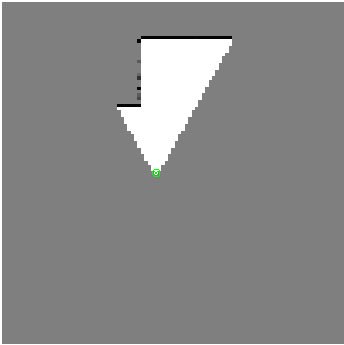
\includegraphics[height=0.4\columnwidth]{Compare_ISM_1.png}
	}
	\subfigure[Map at $t=0$ (approx.)]
		{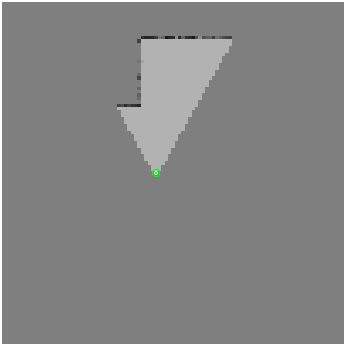
\includegraphics[height=0.4\columnwidth]{Compare_Approx_1.png}
	}
}
\centerline{
	\subfigure[Map at $t=13$ (exact)]
		{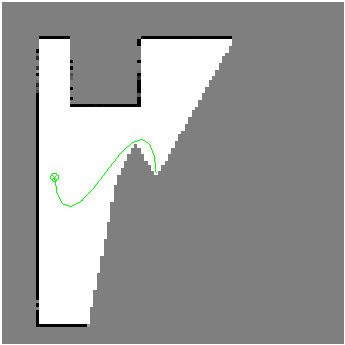
\includegraphics[height=0.4\columnwidth]{Compare_ISM_2.png}
	}
	\subfigure[Map at $t=13$ (approx.)]
		{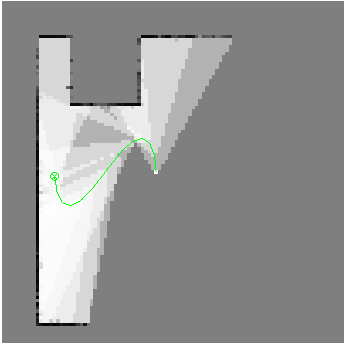
\includegraphics[height=0.4\columnwidth]{Compare_Approx_2.png}
	}
}
\centerline{
	\subfigure[Map at $t=25$ (exact)]
		{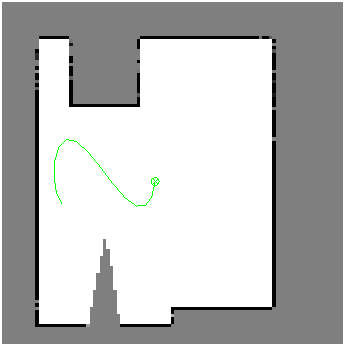
\includegraphics[height=0.4\columnwidth]{Compare_ISM_3.png}
	}
	\subfigure[Map at $t=25$ (approx.)]
		{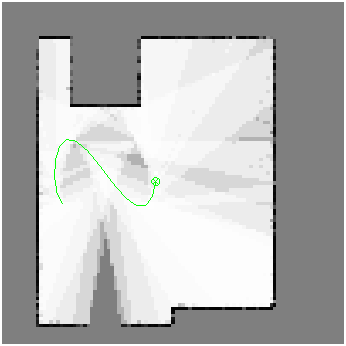
\includegraphics[height=0.4\columnwidth]{Compare_Approx_3.png}
	}
}
\centerline{
	\subfigure[Map at $t=38$ (exact)]
		{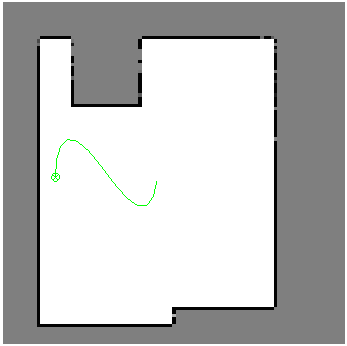
\includegraphics[height=0.4\columnwidth]{Compare_ISM_4.png}
	}
	\subfigure[Map at $t=38$ (approx.)]
		{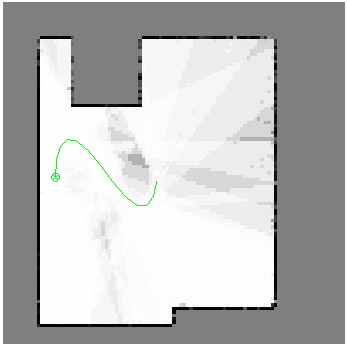
\includegraphics[height=0.4\columnwidth]{Compare_Approx_4.png}
	}
}
\centerline{
	\subfigure[Map at $t=50$ (exact)]
		{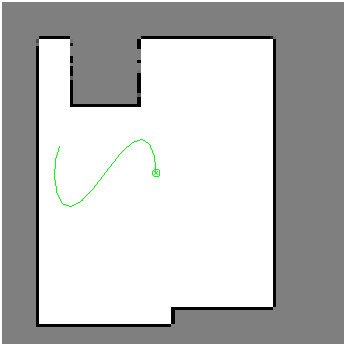
\includegraphics[height=0.4\columnwidth]{Compare_ISM_5.png}
	}
	\subfigure[Map at $t=50$ (approx.)]
		{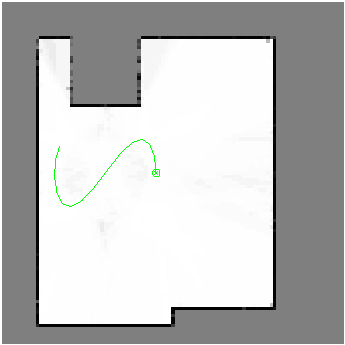
\includegraphics[height=0.4\columnwidth]{Compare_Approx_5.png}
	}
}
\caption{A robot (green crossed circle, green curve of its previous $13$ seconds) measures a room with a Kinect depth sensor. The exact inverse sensor model is compared with an approximate algorithm designed for the Kinect depth sensor. The algorithms update the grid cells from uncertain (grey, $0.5$ occupancy probability) to either occupied (black, $1$ occupancy probability) or free (white, $0$ occupancy probability). Measured cells have occupancy probabilities closer to $0$ or $1$ as more information becomes available, and unmeasured cells remain near $0.5$, or uncertain.
%The exact inverse sensor model approach generates a more accurate result.
}
\label{fig:NumResOccProbs}
\end{figure}

	
\section{Numerical Example}
\label{sec:NumRes}

% It is common practice to approximate\refeqn{InvSenModWithProbDens} with a simplified function, frequently following the structure of the approximate inverse sensor model proposed in~\cite{And09}. The main idea of this approach is that the probability of a cell being occupied ($i$) near a measurement is high (measurement likely hits this cell), ($ii$) between the robot and the measurement is low (measurement passes through this cell), and ($iii$) beyond the measurement is unchanged (the robot cannot measure through a wall/object). The function is based on intuition, not thorough mathematical derivation. In short, this approach simplifies the inverse sensor model at the cost of accuracy.

%The Kinect depth sensor is used as an example, with specifications from~\cite{KhoElb12}. With these parameters and the identical set of measurements, the exact solution is compared with a benchmark algorithm for a Kinect sensor taken from summarized as follows.

The purpose of this section is to compare the proposed exact solution to the inverse sensor model with an approximate algorithm developed for a Microsoft Kinect sensor~\cite{PirRutBisSch11,KhoElb12}, summarized as follows. The probability that the $i$-th grid cell $\mathbf{m}_i$ is occupied conditioned on the measurement ray $z_{t,l}$ (the $l$-th ray at the $t$-th time step) at the pose $X_t$ is the continuous function
\begin{align*}
%\label{eqn:ISM_Approx_1}
&P(\mathbf{m}_i|z_{t,l},X_t)\nonumber\\&=\begin{cases}
0.3+(\frac{k}{\sigma\sqrt{2\pi}}+0.2)e^{-\frac12\left(\frac{\hat z_{l,i}-z_{t,l}}{\sigma}\right)^2}\ &\text{if}\ z_{t,l}\leq \hat z_{l,i},
\\
0.5+\frac{k}{\sigma\sqrt{2\pi}}e^{-\frac12\left(\frac{\hat z_{l,i}-z_{t,l}}{\sigma}\right)^2}\ &\text{if}\ z_{t,l}>\hat z_{l,i},
\end{cases}
\end{align*}
which is based on the expected distance to the cell $\hat z_{l,i}$ with parameters $k=\sigma=0.6$. This follows the structure of the approximate inverse sensor model proposed in~\cite{And09}. The main idea of this approach is that the probability of a cell being occupied (i) near a measurement is high (measurement likely hits this cell), (ii) between the robot and the measurement is low (measurement passes through this cell), and (iii) beyond the measurement is unchanged (the robot cannot measure through a wall/object). 

Then, these probabilities are combined in a weighted fashion such that all measurements rays of scan $Z_t$ simultaneously update the same grid cell in a log-odds format,
\begin{align*}
%\label{eqn:ISM_Approx_2}
&\log\left(\frac{P(\mathbf{m}_i|Z_{t},X_t)}{1-P(\mathbf{m}_i|Z_{t},X_t)}\right)
\nonumber\\&=
\frac1{\sum_{z_{t,l}\in\mathbf{m}_i}\hat z_{l,i}}\sum_{z_{t,l}\in\mathbf{m}_i}\log\left(\frac{P(\mathbf{m}_i|z_{t,l},X_t)}{1-P(\mathbf{m}_i|z_{t,l},X_t)}\hat z_{l,i}\right).
\end{align*}


\subsection{Computation Time}
The proposed ray inverse sensor model is designed to maintain the accuracy of the exact solution with substantial computational improvements.
A $1$-dimensional example is simulated on a Mac desktop computer with $11$ grid cells, $10$ of which are visible to the robot, where the same depth measurement is used for all occupancy grid algorithms.
The computational time of the exact solution is computed in the conventional manner according to \refeqn{InvSenModWithProbDens} in $2.3314$ seconds to obtain the same solution of \refeqn{RayISMAnswer} from \refeqn{Unnormalized} and \refeqn{allEta} in just $0.0027$ seconds, which is $874.77$ times faster.
The approximate ray inverse sensor model completes in $0.0011$ seconds, but this algorithm does not follow a forward sensor model, so the probabilities of the map may be inaccurate.








\subsection{Trajectory Map Building}
In this numerical example, we consider a robot in a two-dimensional environment composed of ten wall edges, and the robot follows a figure-eight curve, then turns around and completes the same curve in the reverse direction.
The map is composed of $100\times100$ square grid cells with edge length of $1$ cm.
A forward sensor model $p(z_t|m,X_t)$~\cite{ThrBurFox05} is constructed according to the specifications of the Kinect sensor~\cite{KhoElb12}, and a pseudo-random measurement scan is sampled at each time step via the inverse transform sampling~\cite{DevBK86}. The same set of measurements updated each second are used with both occupancy grid mapping algorithms to construct the map.

The resulting maps are illustrated in Figure \ref{fig:NumResOccProbs} for both algorithms, where it is shown that the proposed algorithm yields a substantially more accurate and clear map with less uncertainty. To quantify the degree of map uncertainty, we define the entropy of the map as 
\begin{align*}
&H(P(m|X_{1:t},Z_{1:t}))=\nonumber\\
&-\sum_{i=1}^n\big\{P(\mathbf{m}_i|X_{1:t},Z_{1:t})\log P(\mathbf{m}_i|X_{1:t},Z_{1:t})\nonumber\\
&+(1-P(\mathbf{m}_i|X_{1:t},Z_{1:t}))\log(1-P(\mathbf{m}_i|X_{1:t},Z_{1:t}))\big\},
\end{align*}
which is maximized when the probability of occupancy is $0.5$ for all cells (more uncertain), and it is minimized when they are either $0$ or $1$ (less uncertain). 

The change of the map entropy over time, and the entropy of the completed maps, for both methods are depicted in Figure \ref{fig:NumResOccH}. The subfigure (a) illustrates that the proposed exact inverse sensor model exhibits rapid decreases of entropies, and smaller entropies always. The resulting terminal map obtained from the proposed approach, shown in the subfigure (b), has less uncertainty than (c) constructed by the approximate model. In short, the proposed approach is more efficient at extracting information about the environment from the same set of set measurements. 

%The occupancy grids generated by the exact inverse sensor model yield clearer maps with less uncertainty. The entropy of the map from the first measurement to the last is less with the exact model, where sudden decreases correspond to sharp turns in the robot motion. During these turns, the field of view changes greatly, so the information gain from the measurements is large, and therefore the decrease in map uncertainty is also large.


\begin{figure}
\centerline{
	\subfigure[Entropy (black: exact model, green: approx.)]
		{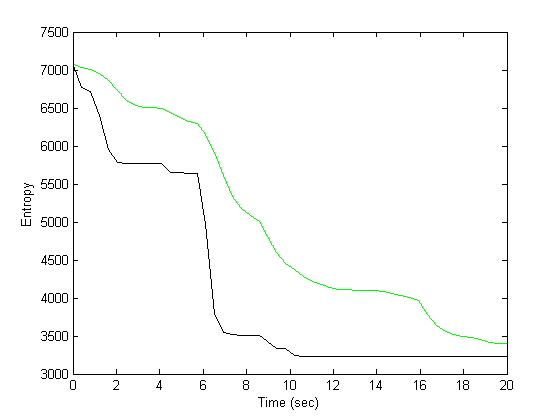
\includegraphics[width=0.7\columnwidth]{EntropyEvolution.png}
	}
}
\centerline{
	\subfigure[Entropy map at $t=50$ (exact)]
		{\hspace*{0.3cm}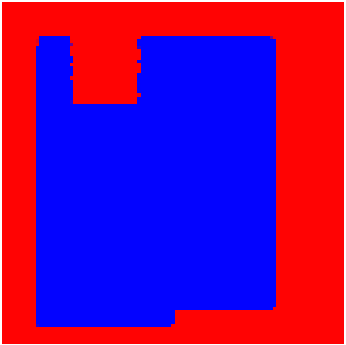
\includegraphics[height=0.4\columnwidth]{Compare_ISM_H.png}\hspace*{0.3cm}
	}
	\subfigure[Entropy map at $t=50$  (approx.)]
		{\hspace*{0.3cm}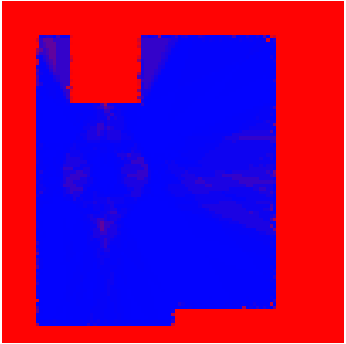
\includegraphics[height=0.4\columnwidth]{Compare_Approx_H.png}\hspace*{0.3cm}
	}
}
\caption{Entropy serves as a measure of uncertainty of the occupancy grid, where more blue regions are more certain, and red regions are more uncertain. The uncertainty is always less when the exact solution is applied.}\label{fig:NumResOccH}
\end{figure}


\section{Preliminary Experimental Results}
\label{sec:ExpRes}
	% Kinect result

%A preliminary experiment shows how the exact inverse sensor model is successfully implemented with the Kinect sensor.

The proposed algorithm is also implemented to range measurements obtained from a Kinect sensor. The map is composed of $200\times200$ square grid cells with edge length of $1$ cm. The parameters for the Kinect sensor are obtained from~\cite{KhoElb12}, and the OpenKinect library is used on a Mac computer to extract range measurements. The Kinect sensor faces walls underneath a work desk, as illustrated in Figures \ref{fig:ExpRes}.(a) and (b). The resulting occupancy grid map and entropy map, obtained from both the proposed algorithm and an approximate model after a single scan~\cite{PirRutBisSch11,KhoElb12}, are also presented. 

\begin{figure}
\centerline{
	\subfigure[Test Setup]
		{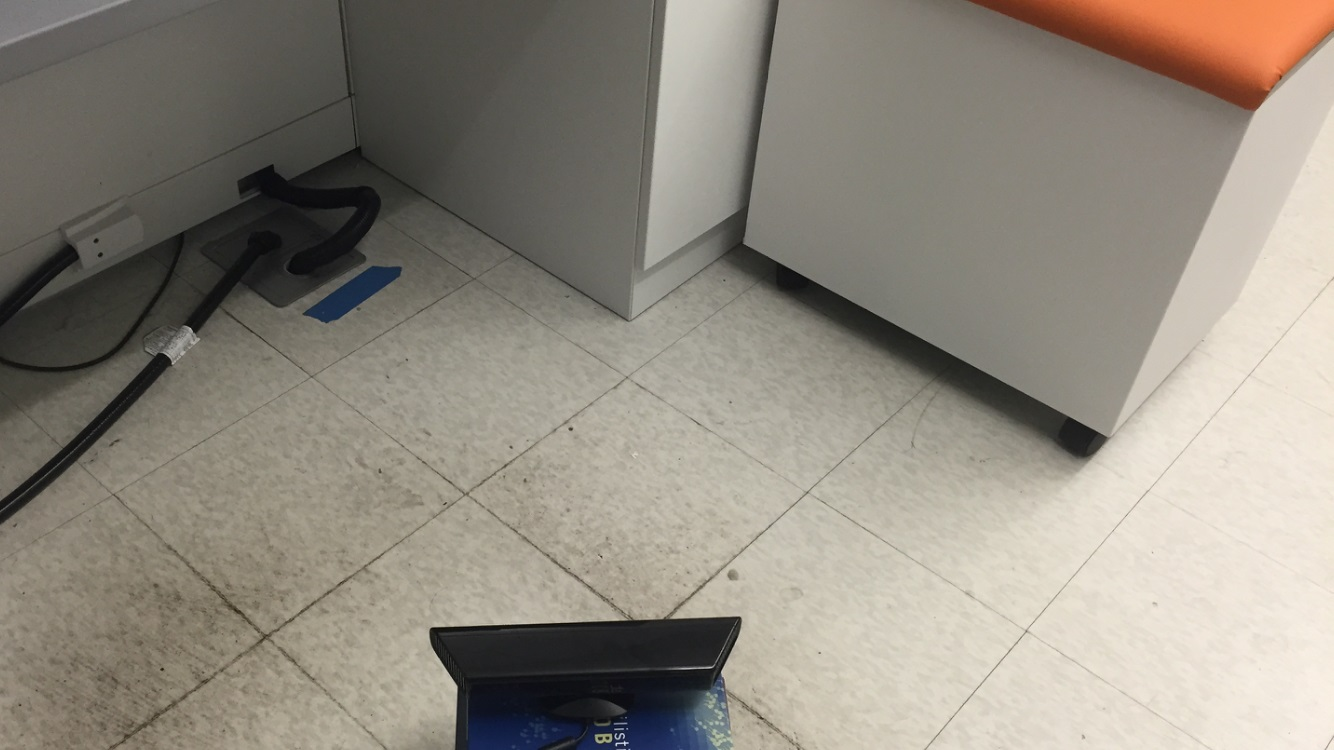
\includegraphics[trim={1.5cm 0 1.5cm 0},clip,height=0.3\columnwidth]{TestSetup.jpg}
	}
	\subfigure[Kinect View]
		{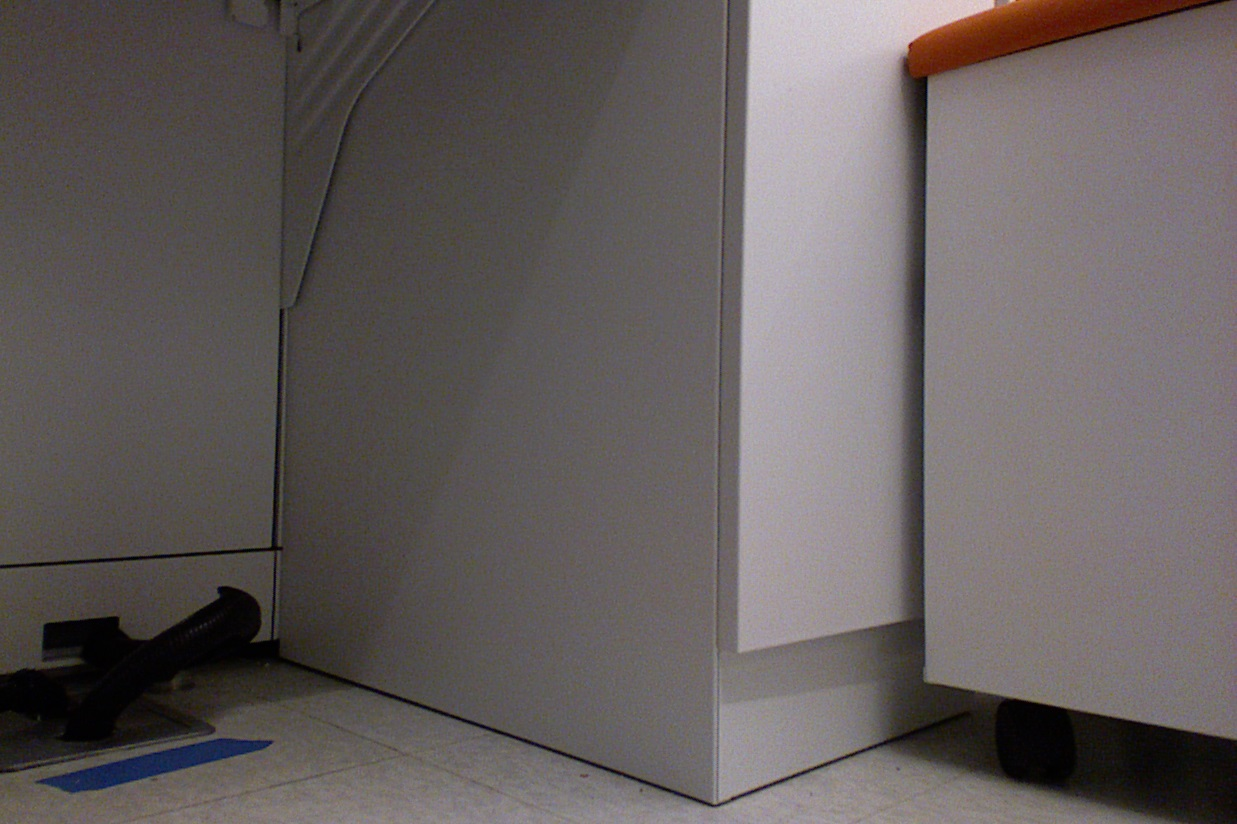
\includegraphics[height=0.3\columnwidth]{KinectView.jpg}
	}
}
\centerline{
	\subfigure[Occupancy map (exact)]
		{
\includegraphics[trim={0 0 0 3cm},clip,height=0.34\columnwidth]{KinectDeskISM.png}
	} 
	\hfill
	\subfigure[Occupancy map (approx.)]
		{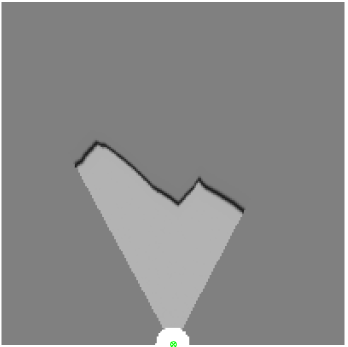
\includegraphics[trim={0 0 0 3cm},clip,height=0.34\columnwidth]{KinectDeskApprox.png}
	}
}
\centerline{
	\subfigure[Entropy map (exact)]
		{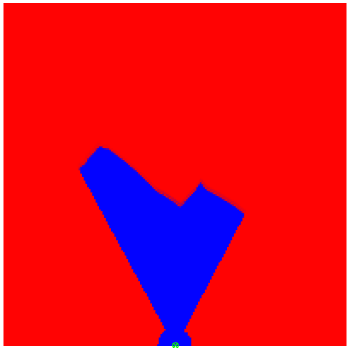
\includegraphics[trim={0 0 0 3cm},clip,height=0.34\columnwidth]{KinectDeskISM_H.png}
	}
	\hfill
	\subfigure[Entropy map (approx.)]
		{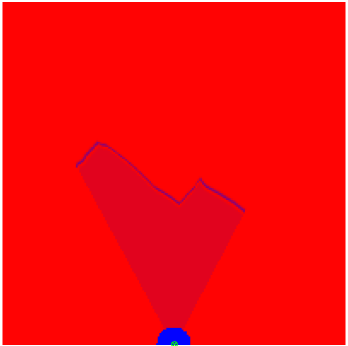
\includegraphics[trim={0 0 0 3cm},clip,height=0.34\columnwidth]{KinectDeskApprox_H.png}
	}
}
\caption{The Kinect captures depth measurements of the underside of a metal desk. The measurement scan serves to update two occupancy grid mapping schemes. The proposed approach, based on the the exact solution of the inverse sensor model, provides an update with substantially less uncertainty than the approximate model update.}\label{fig:ExpRes}
\end{figure}


The proposed approach uses all the information from the measurement scans accurately. After the first scan, the free space has a substantially lower probability of occupancy. Furthermore, the edges of the objects captured by the Kinect are well defined with the proposed approach with an edge thickness of roughly one or two cells, but two or three cells thick with the conventional approach. Additionally, the decrease in entropy is greater with the proposed approach at $-3487$, compared with $-557$ with the approximate inverse sensor model.


\section{Conclusions}

Occupancy grid mapping produces a probabilistic map of occupied space, but each probability is approximated in practice due to the perceived complications of the exact solution.
This paper provides an exact solution to this complicated probability problem using cell occlusion in the forward sensor model. This yields a substantially simpler inverse sensor model, which avoids a potentially harmful Markov assumption that commonly appears in the log-odd ratio formations. The main contribution of this paper is that all of the information available in the measurements and the a priori estimate is extracted and integrated synergistically to generate a more accurate a posteriori map. The numerical and experimental results show that maps using this exact approach are substantially improved. Future study includes developing the presented experimental results further for mapping with a mobile robot, and utilizing the proposed exact inverse sensor model into SLAM and autonomous explorations. 
	



\begin{appendix}
\label{append}


\subsection{Proof of Proposition 1}

\paragraph{Unnormalized Reduced Map Inverse Sensor Model}
For the reduced map of the $l$-th ray, the unnormalized probability that corresponds to the terms without $\eta_{t,l}$ in \refeqn{InvSenModWithProbDens} is given by
\begin{align}
\tilde P&(\mathbf{r}_{l,k}|z_{t,l},X_{1:t},Z_{1:t-1})\nonumber\\
& = \sum_{r\in\mathcal{M}_{k}} p(z_{t,l}|r,X_t) P(r|X_{1:t-1},Z_{1:t-1}).\label{eqn:tildePlk}
\end{align}
Recall $\mathcal{M}_k$ corresponds to the set of maps where the $k$-th cell is occupied. Define a subset $\mathcal{N}_{i,k}\subset \mathcal{M}_k$ for $1\leq i\leq k$ be the set of maps where the $i$-th cell is the first occupied cell. More explicitly, 
\begin{align*}
\mathcal{N}_{i,k} & = \{ r\in\mathcal{M}_k| \mathbf{r}_{l,i+}\}\\
&= \{ r\in\mathcal{M}_k| \mathbf{r}_{l,1}=0,\ldots, \mathbf{r}_{l,i-1}=0, \mathbf{r}_{l,i}=1,
\mathbf{r}_{l,k}=1\}.
\end{align*}
Then, $\mathcal{M}_k$ can be written as $\mathcal{M}_k =\bigcup_{i=1}^{k} \mathcal{N}_{i,k}$. Using this, the summation over $\mathcal{M}_k$ at \refeqn{tildePlk} can be decomposed of the summation over each $\mathcal{N}_{i,k}$ to obtain
\begin{align*}
\tilde P&(\mathbf{r}_{l,k}|z_{t,l},X_{1:t},Z_{1:t-1})\nonumber\\
& = \sum_{i=1}^k\braces{\sum_{r\in\mathcal{N}_{i,k}} p(z_{t,l}|r,X_t) P(r|X_{1:t-1},Z_{1:t-1})}.
\end{align*}
This is motivated by the fact that the forward sensor model $p(z_{t,l}|r,X_t)$ is identical for all maps in $\mathcal{N}_{i,k}$, such that $p(z_{t,l}|r,X_t)=p(z_{t,l}|\mathbf{r}_{l,i+},X_t)$ and it is moved left of the summation to obtain
\begin{align}
\tilde P&(\mathbf{r}_{l,k}|z_{t,l},X_{1:t},Z_{1:t-1})\nonumber\\
& = \sum_{i=1}^k \braces{p(z_{t,l}|\mathbf{r}_{l,i+},X_t) \sum_{r\in\mathcal{N}_{i,k}} P(r|X_{1:t-1},Z_{1:t-1})}.\label{eqn:tildePlk0}
\end{align}
The last term of the above expression corresponds to the a priori probability of $\mathcal{N}_{i,k}$. When $i<k$, it is given by
\begin{align}
\sum_{r\in\mathcal{N}_{i,k}}  &P(r|X_{1:t-1},Z_{1:t-1}) = \bigg\{\prod_{j=0}^{i-1}P(\bar{\mathbf{r}}_{l,j}|X_{1:t-1},Z_{1:t-1})\bigg\}\nonumber\\
 \times &P({\mathbf{r}}_{l,i}|X_{1:t-1},Z_{1:t-1})P({\mathbf{r}}_{l,k}|X_{1:t-1},Z_{1:t-1}),\label{eqn:PNik}
\end{align}
and when $i=k$, 
\begin{align}
\sum_{r\in\mathcal{N}_{k,k}} & P(r|X_{1:t-1},Z_{1:t-1})= \bigg\{\prod_{j=0}^{k-1}P(\bar{\mathbf{r}}_{l,j}|X_{1:t-1},Z_{1:t-1})\bigg\}\nonumber\\
&\quad \times P({\mathbf{r}}_{l,k}|X_{1:t-1},Z_{1:t-1}).\label{eqn:PNkk}
\end{align}
Substituting \refeqn{PNik} and \refeqn{PNkk} into \refeqn{tildePlk0}, we obtain \refeqn{Unnormalized}.



%%Consider the $l$-th measurement ray at time $t$. The $k$-th cell of the reduced map $r$ is denoted $\mathbf{r}_{l,k}$, where $k$ corresponds to cells from map $m$, and is ordered by increasing distance from pose $X_t$.
%%Define $P(\bar{\mathbf{r}}_0)=1$ and $p(z_{t,l}|X_t,\mathbf{r}_0)=0$ for convenience. Then, the probability of occupancy of the first three cells are
%%\begin{align}
%%\label{eqn:tildePk1}
%%&\tilde P(\mathbf{r}_{l,1}|X_t,z_{t,l})\nonumber\\&=\left\{\prod_{j=0}^0P(\bar{\mathbf{r}}_{l,j})\right\}p(z_{t,l}|X_t,\mathbf{r}_{l,1})P(\mathbf{r}_{l,1})
%%,
%%\\
%%&\tilde P(\mathbf{r}_{l,2}|X_t,z_{t,l})\nonumber\\&=
%%P(\mathbf{r}_{l,2})\left\{\prod_{j=0}^0P(\bar{\mathbf{r}}_{l,j})\right\}P(\mathbf{r}_{l,1})p(z_{t,l}|X_t,\mathbf{r}_{l,1})\nonumber\\&\quad+\left\{\prod_{j=0}^1P(\bar{\mathbf{r}}_{l,j})\right\}p(z_{t,l}|X_t,\mathbf{r}_{l,2})P(\mathbf{r}_{l,2})
%%,
%%\\
%%&\tilde P(\mathbf{r}_{l,3}|X_t,z_{t,l})\nonumber\\&=
%%P(\mathbf{r}_{l,3})\sum_{i=1}^2
%%\left\{\prod_{j=0}^{i-1}P(\bar{\mathbf{r}}_{l,j})\right\}P(\mathbf{r}_{l,i})p(z_{t,l}|\mathbf{r}_{l,i},X_t)\nonumber\\
%%&+\left\{\prod_{j=0}^2P(\bar{\mathbf{r}}_{l,j})\right\}p(z_{t,l}|X_t,\mathbf{r}_{l,3})P(\mathbf{r}_{l,3})
%%,
%%\end{align}
%%respectively. This is generalized to the arbitrary $k$-th cell as
%%\begin{align}
%%\label{eqn:GenSol}
%%&\tilde P(\mathbf{r}_k|X,z)
%%\nonumber\\&=P(\mathbf{r}_{l,k})\sum_{i=1}^{k-1}\left\{\prod_{j=0}^{i-1}P(\bar{\mathbf{r}}_{l,j})\right\}p(z_{t,l}|\mathbf{r}_{l,i},X_t)P(\mathbf{r}_{l,i})
%%\nonumber\\&\quad+
%%\left\{\prod_{j=0}^{k-1}P(\bar{\mathbf{r}}_{l,j})\right\}p(z_{t,l}|\mathbf{r}_{l,k},X_t)P(\mathbf{r}_{l,k}),
%%\end{align}
%%where special cases when the lower bound of a summation is greater than the upper bound results in a summation value of $0$.
%%
%%\emph{Proof by Induction of the Reduced Inverse Sensor Model \refeqn{GenSol}}
%%Consider the base case when $k=1$ such that the $k$-th cell would block all others. This corresponds to $\tilde P(\mathbf{r}_{l,1}|X_t,z_{t,l})=p(z_{t,l}|X_t,\mathbf{r}_{l,1})P(\mathbf{r}_{l,1})$, which is equivalent to \refeqn{tildePk1}.
%%Next, the inductive step is solved for the $k+1$ index,
%%\begin{align}
%%\label{eqn:GenSol_InductiveStep}
%%\tilde P(\mathbf{r}_{l,k+1}|X_t,z_{t,l})
%%%&=
%%%P(\mathbf{r}_{k+1})\sum_{r:r({k+1})=\mathbf{r}_{k+1}}p(z|X,r)P(r)\nonumber
%%%\\
%%%&=P(\mathbf{r}_{k+1})\{
%%%P(\mathbf{r}_1)\sum_{\substack{r:r(1)=\mathbf{r}_1\\r({k+1})=\mathbf{r}_{k+1}}}p(z|X,r)P(r|\mathbf{r}_1,\mathbf{r}_{k+1})
%%%\nonumber
%%%\\
%%%&\quad
%%%+P(\bar{\mathbf{r}}_1)\sum_{\substack{r:r(1)=\bar{\mathbf{r}}_1\\r({k+1})=\mathbf{r}_{k+1}}}p(z|X,r)P(r|\bar{\mathbf{r}}_1,\mathbf{r}_{k+1})\}
%%%\nonumber
%%%\\
%%&=P(\mathbf{r}_{l,k+1})\bigg\{
%%P(\bar{\mathbf{r}}_{l,0})P(\mathbf{r}_{l,1})p(z_{t,l}|X_t,\mathbf{r}_{l,1})+\nonumber\\&\quad P(\bar{\mathbf{r}}_{l,0})P(\bar{\mathbf{r}}_{l,1})P(\mathbf{r}_{l,2})p(z_{t,l}|X_t,\mathbf{r}_{l,2})+...\nonumber
%%\\
%%&\quad +\left(
%%P(\bar{\mathbf{r}}_{l,0})P(\bar{\mathbf{r}}_{l,1})...P(\bar{\mathbf{r}}_{l,k-1})
%%\right)\nonumber
%%\\
%%&\quad\times P(\mathbf{r}_{l,k})p(z_{t,l}|X_t,\mathbf{r}_{l,k})\bigg\}\nonumber
%%\\
%%&\quad
%%+\left(
%%P(\bar{\mathbf{r}}_{l,0})P(\bar{\mathbf{r}}_{l,1})...P(\bar{\mathbf{r}}_{l,k})
%%\right)\nonumber
%%\\
%%&\quad\times p(z_{t,l}|X_t,\mathbf{r}_{l,k+1})P(\mathbf{r}_{l,k+1})\nonumber
%%\\
%%&=P(\mathbf{r}_{l,k+1})\sum_{i=1}^{k}\left\{\prod_{j=0}^{i-1}P(\bar{\mathbf{r}}_{l,j})\right\}\nonumber
%%\\
%%&\quad\times p(z_{t,l}|\mathbf{r}_{l,i},X_t)P(\mathbf{r}_{l,i})\nonumber\\&\quad
%%+
%%\left\{\prod_{j=0}^{k}P(\bar{\mathbf{r}}_{l,j})\right\}\nonumber
%%\\
%%&\quad\times p(z_{t,l}|X_t,\mathbf{r}_{l,k+1})P(\mathbf{r}_{l,k+1})
%%.
%%\end{align}

\paragraph{Complement of the Unnormalized Reduced Map Inverse Sensor Model}
An analytic expression for the complement of the unnormalized inverse sensor model is also required  for obtaining the normalizer of the $l$-th ray at time $t$, namely $\eta_{t,l}$. Let $\bar{\mathcal{M}}_k$ be the set of maps where the $k$-th cell is unoccupied, i.e., $\bar{\mathcal{M}}_k = \{ r\in\{0,1\}^{n_{r,l}}\,|\, \mathbf{r}_{l,k}=0\}$. Similar to \refeqn{tildePlk},
\begin{align}
\tilde P&(\bar{\mathbf{r}}_{l,k}|z_{t,l},X_{1:t},Z_{1:t-1})\nonumber\\
& = \sum_{r\in\bar{\mathcal{M}}_{k}} p(z_{t,l}|r,X_t) P(r|X_{1:t-1},Z_{1:t-1}).\label{eqn:tildePbarlk}
\end{align}

Let $\bar{\mathcal{N}}_{i,k}\subset \bar{\mathcal{M}}_k $ for $1\leq i\leq n_{r,l}$ and $i\neq k$ be the set of maps where the $i$-th cell is the first occupied cell. More explicitly, 
\begin{align*}
\bar{\mathcal{N}}&_{i,k}\nonumber\\&=\{r\in\bar{\mathcal{M}}_k\,|\, \mathbf{r}_{l,1}=0,\ldots,\mathbf{r}_{l,i-1}=0,
\mathbf{r}_{l,i}=1,\mathbf{r}_{l,k}=0\}.
\end{align*}
Then, we have $\bar{\mathcal{M}}_k=\bigcup_{\substack{i=1\\i\neq k}}^{n_{r,l}} \bar{\mathcal{N}}_{i,k}$. Note that the forward sensor model $p(z_{t,l}|r,X_t)$ is identical for any maps in $\bar{\mathcal{N}}_{i,k}$, such that $p(z_{t,l}|r,X_t)=p(z_{t,l}|\mathbf{r}_{l,i+},X_t)$. Similar to \refeqn{tildePlk0},
\begin{align}
\tilde P&(\bar{\mathbf{r}}_{l,k}|z_{t,l},X_{1:t},Z_{1:t-1})\nonumber\\
& = \sum_{\substack{i=1\\i\neq k}}^{n_{r,l}} \braces{p(z_{t,l}|\mathbf{r}_{l,i+},X_t) \sum_{r\in\bar{\mathcal{N}}_{i,k}} P(r|X_{1:t-1},Z_{1:t-1})},\label{eqn:tildePbarlk0}
\end{align}
where the last term corresponds to the a priori probability of $\bar{\mathcal{N}}_{i,k}$. When $i<k$, it is given by
\begin{align}
\sum_{r\in\bar{\mathcal{N}}_{i,k}} & P(r|X_{1:t-1},Z_{1:t-1}) = \bigg\{\prod_{j=0}^{i-1}P(\bar{\mathbf{r}}_{l,j}|X_{1:t-1},Z_{1:t-1})\bigg\}\nonumber\\
&\quad \times P({\mathbf{r}}_{l,i}|X_{1:t-1},Z_{1:t-1})P(\bar{\mathbf{r}}_{l,k}|X_{1:t-1},Z_{1:t-1}),\label{eqn:PbarNik1}
\end{align}
and when $k<i$,
\begin{align}
\sum_{r\in\bar{\mathcal{N}}_{i,k}} & P(r|X_{1:t-1},Z_{1:t-1}) = \bigg\{\prod_{j=0}^{i-1}P(\bar{\mathbf{r}}_{l,j}|X_{1:t-1},Z_{1:t-1})\bigg\}\nonumber\\
&\quad \times P({\mathbf{r}}_{l,i}|X_{1:t-1},Z_{1:t-1}).\label{eqn:PbarNik2}
\end{align}
Substituting \refeqn{PbarNik1} and \refeqn{PbarNik2} into \refeqn{tildePbarlk0}, we obtain
\begin{align}
\tilde P &(\bar{\mathbf{r}}_k|z_{t,l},X_{1:t},Z_{1:t-1})
=P(\bar{\mathbf{r}}_{l,k}|X_{1:t-1},Z_{1:t-1})\nonumber\\
&\quad\times \bigg[\sum_{i=1}^{k-1}\bigg\{\prod_{j=0}^{i-1}P(\bar{\mathbf{r}}_{l,j}|X_{1:t-1},Z_{1:t-1})\bigg\}\nonumber\\
&\quad\times p(z_{t,l}|\mathbf{r}_{l,i+},X_t)P(\mathbf{r}_{l,i}|X_{1:t-1},Z_{1:t-1})\bigg]
\nonumber
\\
&\quad
+
\bigg[\sum_{i=k+1}^{n_{r,l}+1}\bigg\{\prod_{j=0}^{i-1}P(\bar{\mathbf{r}}_{l,j}|X_{1:t-1},Z_{1:t-1})\bigg\}\nonumber\\
&\quad\times p(z_{t,l}|\mathbf{r}_{i+},X_t)P(\mathbf{r}_{l,i}|X_{1:t-1},Z_{1:t-1})\bigg],\label{eqn:tildePbar}
\end{align}
where $p(z_{t,l}|\mathbf{r}_{(n_r+1)+},X_t)$ corresponds to the forward sensor model of maximum reading and $P(\mathbf{r}_{l,n_{r,l}+1}|X_{1:t-1},Z_{1:t-1})=1$ for convenience for the empty map case.

% ADD: where it is considered $P(\bar{\mathbf{r}}_{l,0}|X_{1:t-1},Z_{1:t-1})=P(\mathbf{r}_{l,n_r+1}|X_{1:t-1},Z_{1:t-1})=1$ and $p(z_{t,l}|\mathbf{r}_{l,(n_r+1)+},X_t)$

%%The unnormalized complement of the $k$-th cell inverse sensor model, namely $\tilde P(\bar{\mathbf{r}}_k|X,z)$, is required to solve for $\eta$ based on \refeqn{allEta}.
%%Consider the complement of the occupancy of the first and second cells, i.e.,
%%\begin{align}
%%\label{eqn:InvSenModknot1}
%%\tilde P(\bar{\mathbf{r}}_{l,1}|X_t,z_{t,l})
%%&=P(\bar{\mathbf{r}}_{l,1})
%%\bigg\{P(\mathbf{r}_{l,2})
%%p(z_{t,l}|X_t,\mathbf{r}_{l,2})\nonumber\\&\quad
%%+P(\bar{\mathbf{r}}_{l,2})P(\mathbf{r}_{l,3})p(z_{t,l}|X_t,\mathbf{r}_{l,3})+...\nonumber\\&\quad+\prod_{j=2}^{n_r-1}P(\bar{\mathbf{r}}_{l,j})P(\mathbf{r}_{l,n_r})p(z_{t,l}|X_t,\mathbf{r}_{l,n_r})
%%\bigg\}\nonumber
%%\\
%%&=\sum_{i=2}^{n_r}
%%\left\{\prod_{j=0}^{i-1}P(\bar{\mathbf{r}}_{l,j})
%%\right\}P(\mathbf{r}_{i})p(z_{t,l}|X_t,\mathbf{r}_{l,i}).
%%\\
%%\label{eqn:InvSenModknot2}
%%\tilde P(\bar{\mathbf{r}}_{l,2}|X_t,z_{t,l})
%%%&=\sum_{r:r(2)=\bar{\mathbf{r}}_2}p(z|X,r)P(r)\nonumber
%%%\\
%%%&=P(\bar{\mathbf{r}}_2)\sum_{r:r(2)=\bar{\mathbf{r}}_2}p(z|X,r)P(r|\bar{\mathbf{r}}_2)\nonumber
%%%\\
%%%&=P(\bar{\mathbf{r}}_2)\left\{P(\mathbf{r}_1)
%%%\sum_{\substack{r:r(1)=\mathbf{r}_1\\r(2)=\bar{\mathbf{r}}_2}}p(z|X,r)P(r|\mathbf{r}_1,\bar{\mathbf{r}}_2)
%%%+P(\bar{\mathbf{r}}_1)\sum_{\substack{r:r(1)=\bar{\mathbf{r}}_1\\r(2)=\bar{\mathbf{r}}_2}}p(z|X,r)P(r|\bar{\mathbf{r}}_1,\bar{\mathbf{r}}_2)
%%%\right\}\nonumber
%%%\\
%%%&=P(\bar{\mathbf{r}}_2)
%%%\{
%%%P(\mathbf{r}_1)p(z|X,\mathbf{r}_1)
%%%+P(\bar{\mathbf{r}}_1)
%%%[
%%%P(\mathbf{r}_3)\sum_{\substack{r:r(1)=\bar{\mathbf{r}}_1\\r(2)=\bar{\mathbf{r}}_2\\r(3)=\mathbf{r}_3}}p(z|X,r)P(r|\bar{\mathbf{r}}_1,\bar{\mathbf{r}}_2,\mathbf{r}_3)\nonumber
%%%\\
%%%&\quad
%%%+
%%%P(\bar{\mathbf{r}}_3)\sum_{\substack{r:r(1)=\bar{\mathbf{r}}_1\\r(2)=\bar{\mathbf{r}}_2\\r(3)=\bar{\mathbf{r}}_3}}p(z|X,r)P(r|\bar{\mathbf{r}}_1,\bar{\mathbf{r}}_2,\bar{\mathbf{r}}_3)
%%%]
%%%\}\nonumber
%%%\\
%%&=P(\bar{\mathbf{r}}_{l,2})
%%\bigg\{
%%P(\mathbf{r}_{l,1})p(z_{t,l}|X_t,\mathbf{r}_{l,1})\nonumber\\&\quad
%%+
%%P(\bar{\mathbf{r}}_{l,1})P(\mathbf{r}_{l,3})p(z_{t,l}|X_t,\mathbf{r}_{l,3})\nonumber\\&\quad
%%+P(\bar{\mathbf{r}}_{l,1})P(\bar{\mathbf{r}}_{l,3})P(\mathbf{r}_{l,4})\nonumber\\&\qquad\times p(z_{t,l}|X_t,\mathbf{r}_{l,4})+...\nonumber
%%\\
%%&\quad+\prod_{j=1,j\neq2}^{n_r-1}P(\bar{\mathbf{r}}_{l,j})P(\mathbf{r}_{l,n_r})p(z_{t,l}|X_t,\mathbf{r}_{l,n_r})
%%\bigg\}\nonumber
%%\\
%%&=
%%P(\bar{\mathbf{r}}_{l,2})\sum_{i=1}^{1}
%%\left\{
%%\prod_{j=0}^{i-1}P(\bar{\mathbf{r}}_{l,j})\right\}\nonumber\\&\quad\times P(\mathbf{r}_{l,i})p(z_{t,l}|X_t,\mathbf{r}_{l,i})\nonumber\\&\quad+\sum_{i=3}^{n_r}
%%\left\{
%%\prod_{j=0}^{i-1}P(\bar{\mathbf{r}}_{l,j})\right\}\nonumber\\&\quad\times P(\mathbf{r}_{l,i})p(z_{t,l}|X_t,\mathbf{r}_{l,i})
%%.
%%\end{align}
%%
%%
%%
%%In general, the $k$-th unnormalized inverse sensor model complement is
%%\begin{align}
%%\label{eqn:ComplGenSol}
%%\tilde P&(\bar{\mathbf{r}}_{l,k}|X,z)\nonumber\\&=P(\bar{\mathbf{r}}_{l,k})\sum_{i=1}^{k-1}
%%\left\{
%%\prod_{j=0}^{i-1}P(\bar{\mathbf{r}}_{l,j})\right\}P(\mathbf{r}_{l,i})p(z_{t,l}|X_t,\mathbf{r}_{l,i})\nonumber\\&\quad
%%+\sum_{i=k+1}^{n_r}
%%\left\{
%%\prod_{j=0}^{i-1}P(\bar{\mathbf{r}}_{l,j})\right\}P(\mathbf{r}_{l,i})p(z_{t,l}|X_t,\mathbf{r}_{l,i})
%%,
%%\end{align}
%%where special cases when the lower bound of a summation is greater than the upper bound results in a summation value of $0$.
%%
%%\paragraph{Proof by Induction of the Complement of the Reduced Inverse Sensor Model \refeqn{ComplGenSol}}
%%The base case for the occupancy probability is obtain directly from substituting $k=1$ into \refeqn{ComplGenSol} to obtain $\tilde P(\bar{\mathbf{r}}_1|X,z)=\sum_{i=2}^{n_r}\left\{\prod_{j=0}^{i-1}P(\bar{\mathbf{r}}_{l,j})\right\}P(\mathbf{r}_{i})p(z_{t,l}|X_t,\mathbf{r}_{l,i})$.
%%The inductive step is solved for the $k+1$ index,
%%\begin{align}
%%\tilde P&(\bar{\mathbf{r}}_{l,k+1}|X_t,z_{t,l})\nonumber\\
%%%&=P(\bar{\mathbf{r}}_{k+1})
%%%\{
%%%[
%%%P(\mathbf{r}_1)p(z|X,\mathbf{r}_1)
%%%+
%%%P(\bar{\mathbf{r}}_1)P(\mathbf{r}_2)p(z|X,\mathbf{r}_2)
%%%+P(\bar{\mathbf{r}}_1)P(\bar{\mathbf{r}}_2)P(\mathbf{r}_3)p(z|X,\mathbf{r}_3)+...\nonumber
%%%\\
%%%&\quad
%%%+P(\bar{\mathbf{r}}_1)P(\bar{\mathbf{r}}_2)...P(\bar{\mathbf{r}}_{k-1})P(\mathbf{r}_k)p(z_{t,l}|\mathbf{r}_k,X_t)
%%%]\nonumber
%%%\\
%%%&\quad
%%%+
%%%P(\bar{\mathbf{r}}_{k+1})^{-1}[
%%%P(\bar{\mathbf{r}}_1)P(\bar{\mathbf{r}}_2)...P(\bar{\mathbf{r}}_{k+1})P(\mathbf{r}_{k+2})p(z|X,\mathbf{r}_{k+2})+...
%%%\nonumber
%%%\\
%%%&\quad
%%%+P(\bar{\mathbf{r}}_1)P(\bar{\mathbf{r}}_2)...P(\bar{\mathbf{r}}_{n_r-1})P(\mathbf{r}_{n_r})p(z|X,\mathbf{r}_{n_r})
%%%]
%%%\}\nonumber
%%%\\
%%&=
%%P(\bar{\mathbf{r}}_{l,k+1})\nonumber
%%\\
%%&\quad
%%\times\bigg[
%%\left\{\prod_{j=0}^{0}P(\bar{\mathbf{r}}_{l,j})\right\}P(\mathbf{r}_{l,1})p(z_{t,l}|X_t,\mathbf{r}_{l,1})\nonumber
%%\\
%%&\quad
%%+
%%\left\{\prod_{j=0}^{1}P(\bar{\mathbf{r}}_{l,j})\right\}P(\mathbf{r}_{l,2})p(z_{t,l}|X_t,\mathbf{r}_{l,2})\nonumber
%%\\
%%&\quad
%%+\left\{\prod_{j=0}^{2}P(\bar{\mathbf{r}}_{l,j})\right\}P(\mathbf{r}_{l,3})p(z_{t,l}|X_t,\mathbf{r}_{l,3})+...\nonumber
%%\\
%%&\quad
%%+\left\{\prod_{j=0}^{k-1}P(\bar{\mathbf{r}}_{l,j})\right\}P(\mathbf{r}_{l,k})p(z_{t,l}|\mathbf{r}_{l,k},X_t)
%%\bigg]\nonumber
%%\\
%%&\quad
%%+
%%\bigg[
%%\left\{\prod_{j=0}^{k+1}P(\bar{\mathbf{r}}_{l,j})\right\}P(\mathbf{r}_{l,k+2})p(z_{t,l}|X_t,\mathbf{r}_{l,k+2})+...\nonumber
%%\\
%%&\quad
%%+\left\{\prod_{j=0}^{n_r-1}P(\bar{\mathbf{r}}_{l,j})\right\}P(\mathbf{r}_{l,n_r})p(z_{t,l}|X_t,\mathbf{r}_{l,n_r})
%%\bigg]
%%\nonumber
%%\\
%%&=P(\bar{\mathbf{r}}_{l,k+1})\sum_{i=1}^{k}
%%\left\{
%%\prod_{j=0}^{i-1}P(\bar{\mathbf{r}}_{l,j})\right\}P(\mathbf{r}_{l,i})p(z_{t,l}|X_t,\mathbf{r}_{l,i})\nonumber
%%\\
%%&\quad
%%+\sum_{i=k+2}^{n_r}
%%\left\{
%%\prod_{j=0}^{i-1}P(\bar{\mathbf{r}}_{l,j})\right\}P(\mathbf{r}_{l,i})p(z_{t,l}|X_t,\mathbf{r}_{l,i})
%%.
%%\end{align}

\paragraph{Normalizer}
We have 
\begin{align*}
P(\mathbf{r}_{l,k}|z_{t,l},X_{1:t},Z_{1:t-1})+
P(\bar{\mathbf{r}}_{l,k}|z_{t,l},X_{1:t},Z_{1:t-1})=1.
\end{align*}
Since they share the same normalizer $\eta_{t,l}$, this implies 
\begin{align*}
&\eta_{t,l}\nonumber\\&=[\tilde P(\mathbf{r}_{l,k}|z_{t,l},X_{1:t},Z_{1:t-1})+
\tilde P(\bar{\mathbf{r}}_{l,k}|z_{t,l},X_{1:t},Z_{1:t-1})]^{-1}.
\end{align*}
Substituting \refeqn{Unnormalized} and \refeqn{tildePbar}, and rearranging, we obtain \refeqn{allEta}.
%
%\begin{align}
%\eta_{t,l}
%&=\bigg[\sum_{i=1}^{n_r}\left\{\prod_{j=0}^{i-1}P(\bar{\mathbf{r}}_{l,j}|X_{1:t-1},Z_{1:t-1})\right\}\nonumber\\&\quad\times p(z_{t,l}|\mathbf{r}_{i+},X_t)P(\mathbf{r}_i|X_{1:t-1},Z_{1:t-1})\bigg]^{-1},
%\end{align}
%which is independent of the reduced cell index $k$.


\end{appendix}



\bibliography{BibSources}
\bibliographystyle{IEEEtran}


\end{document}




\end{document}
